\chapter{Role of astrophysical modeling on dark matter halo relaxation response at redshifts $z=0$ and $z=1$}
\label{chap:physvar_z01}

In this chapter, we begin by exploring the relaxation response at an earlier redshift in the IllustrisTNG reference simulation. This allows us to understand how the different galactic processes occurring at earlier times affect dark matter halo relaxation. Following this, we examine variations in the baryonic prescriptions in the CAMELS and EAGLE simulations.

\subsection{Early epoch in IllustrisTNG simulations}
\label{sec:res-itng-z01}
In this section, we systematically investigate the relaxation in the IllustrisTNG simulation at an earlier redshift of $z = 1$ and compare it to the present redshift of $z = 0$. While present epoch haloes are sampled only by their masses at the present time, we consider three different methods for sampling the early epoch haloes. This results in four distinct sets of halo samples:

\begin{enumerate}
\item $z=1$ haloes sampled by their masses at $z=1$.
\item $z=1$ haloes sampled by the masses of their descendants at $z=0$. This is done using SubLink merger tree catalogues to trace the most massive progenitors of the $z=0$ haloes. Note that not all haloes with a given mass at the present time have progenitors with the same mass at $z=1$.
\item $z=1$ haloes sampled by their masses at $z=1$, but the mass bins are defined by the median masses of the most massive progenitors of the $z=0$ haloes.
\item $z=0$ haloes sampled by their masses at $z=0$.
\end{enumerate}

For each of these four sets of halo samples, the overall relaxation relation ($r_f/r_i$ vs $M_i/M_f$) is shown in \figref{fig:fit-view-mass-indep}. We find that, for a given halo mass, relaxation is usually stronger at the earlier epoch (top left panel) compared to the present time $z=0$ (bottom right panel). In both cases, the trend in relaxation with halo mass is similar, with the strongest relaxation observed in $10^{12} \Mh$ haloes. Interestingly, cluster-scale haloes with masses of $10^{14} \Mh$ at redshift $z=1$ exhibit significant relaxation, unlike clusters of similar size at the present time.

The progenitors at redshift $z=1$ of the same haloes found at $z=0$ show even stronger relaxation, especially in Milky Way-scale and larger haloes, as shown in the top right panel of \figref{fig:fit-view-mass-indep}. The relaxation follows the simple quasi-adiabatic model \eqref{eq:chi-linear} with $q=0.33$ among larger cluster-scale ($10^{14} \Mh$) haloes, while group-scale haloes are consistent with the second-order polynomial relation proposed by Abadi et al. (2010) \cite{2010MNRAS.407..435A}. In the bottom left panel, the relaxation relation is shown for all haloes within a narrow mass bin around the median mass of the progenitors of the haloes selected at $z=0$. Notice that the relaxation relation shifts further lower in Milky Way-scale haloes and smaller clusters with the inclusion of those additional haloes.

\begin{figure}[htbp]
\centering
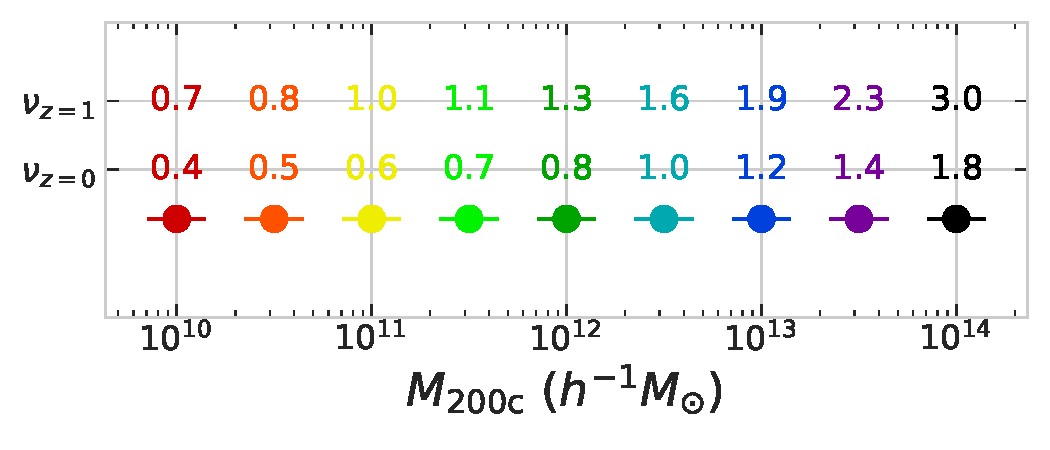
\includegraphics[width=0.49\linewidth]{plots/Mass_bin_labels_z.pdf}
\caption{Representative colors denoting each of the halo mass bins. The numbers in the figure indicate the corresponding values of peak heights $\nu$ at redshifts $z=0$ and $z=1$.}
\label{fig:mass_bin_label}
\end{figure}

\begin{figure*}
\centering
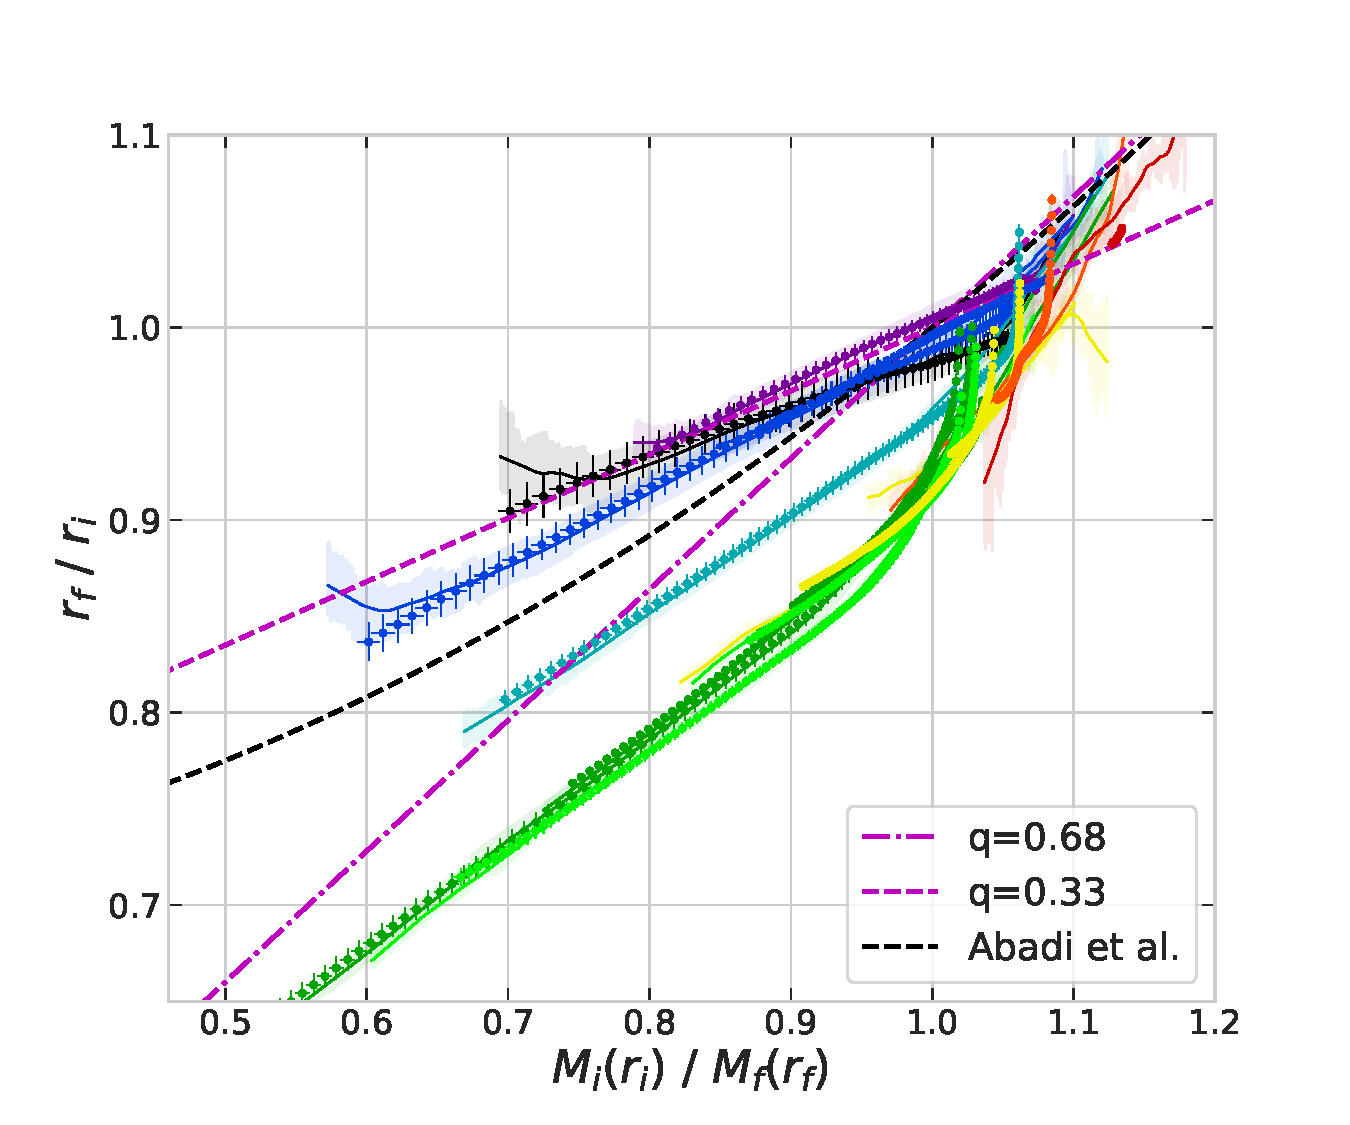
\includegraphics[width=0.48\linewidth]{plots/fit_view_M_T_snap049.pdf}
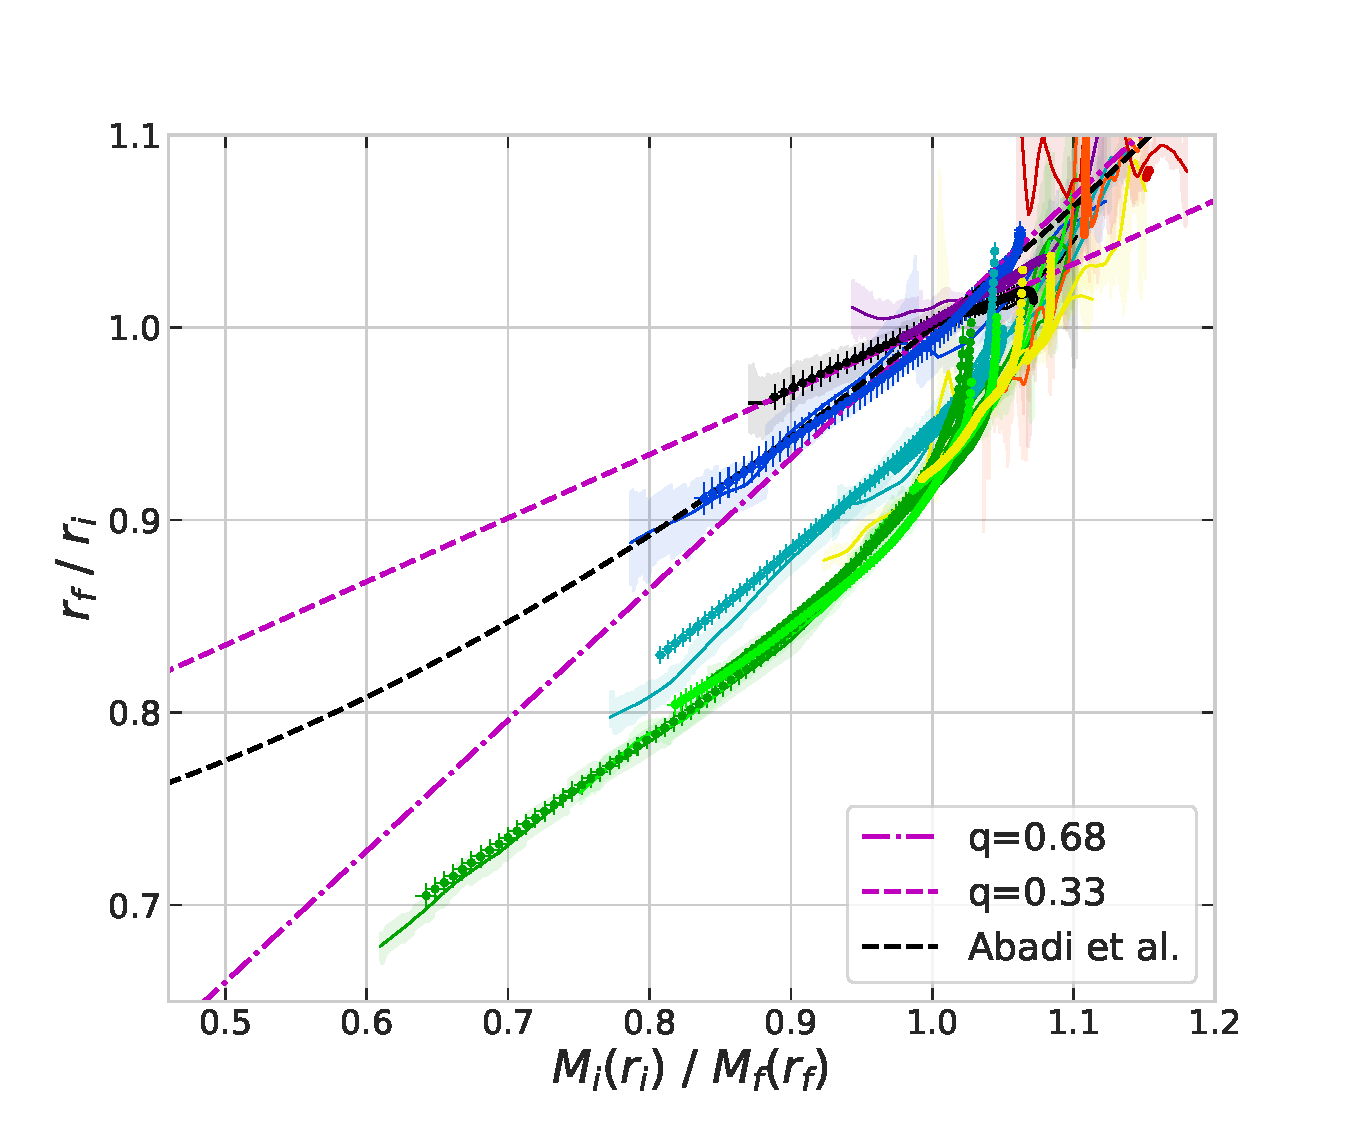
\includegraphics[width=0.48\linewidth]{plots/fit_view_M_T_snap049_smpl98.pdf}
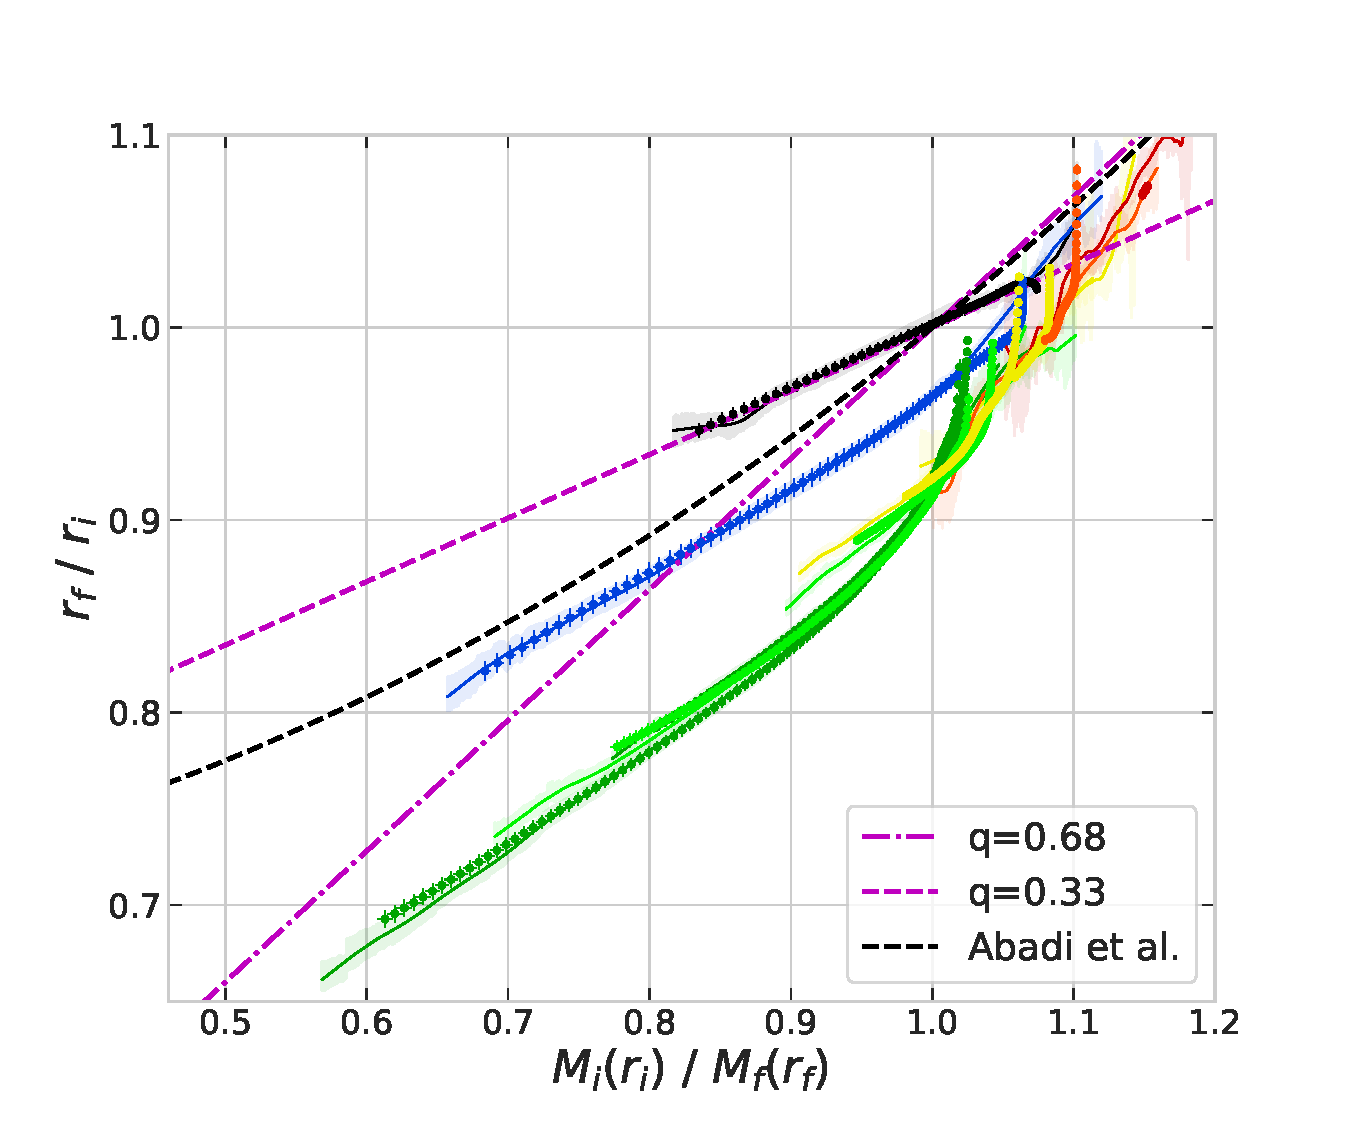
\includegraphics[width=0.48\linewidth]{plots/fit_view_M_T_snap049_smpl98_allHalsMrange.pdf}
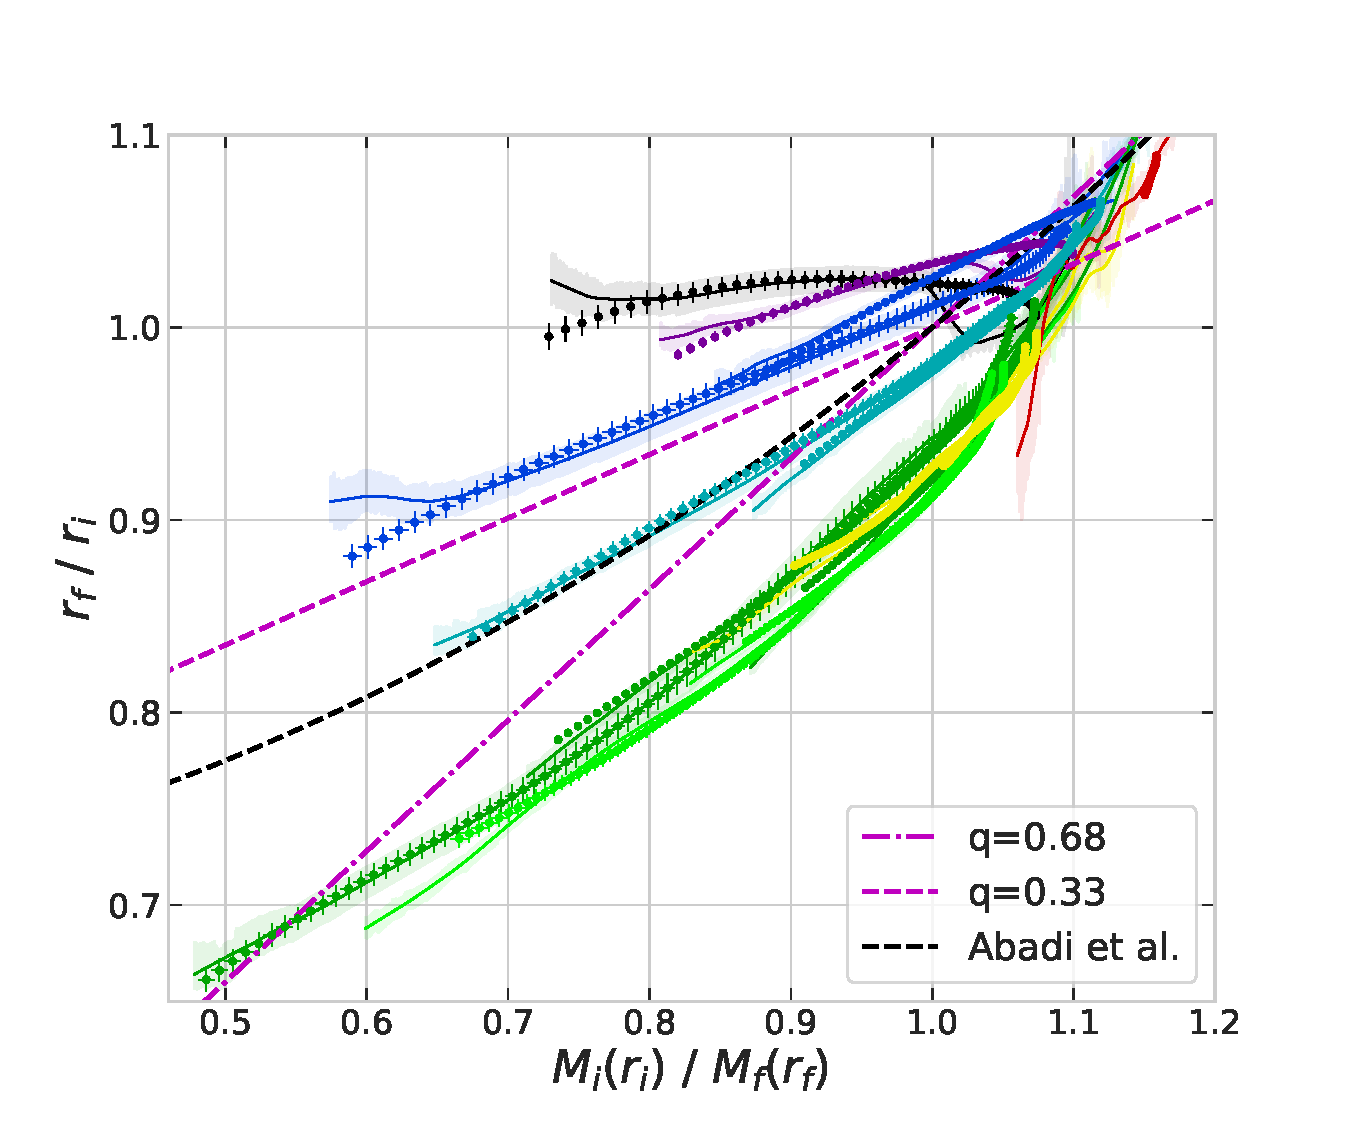
\includegraphics[width=0.48\linewidth]{plots/fit_view_M_T_snap098.pdf}
\caption{The stacked relation between relaxation ratio and mass ratio as a function of halo mass in IllustrisTNG at $z=0$ \emph{(bottom right panel)} and $z=1$ \emph{(other panels)}. In the top right panel, relaxation is shown at $z=1$ for the progenitors of the haloes selected at $z=0$. In the second row, left panel, relaxation is shown at different mass bins at $z=1$, indicated by corresponding mass bins at $z=0$. Points represent stacks over fixed halo-centric distances, and solid lines represent stacks over fixed mass ratios. The color-coding follows Fig.~\ref{fig:mass_bin_label}. The quasi-adiabatic relaxation model \eqref{eq:chi-linear} with $q=0.68$ and $q=0.33$ are shown by the dot-dashed and dashed purple lines, respectively, in each panel.}
\label{fig:fit-view-mass-indep}
\end{figure*}

In Velmani \& Paranjape (2023) \cite{2023Velmani&Paranjape}, we proposed a locally linear model of the relaxation relation as follows:
\begin{align}
\label{eq:chi-linear-q0}
\frac{r_f}{r_i} - 1 &= q_1(r_f) \left[ \frac{M_i(r_i)}{M_f(r_f)} - 1 \right] + q_0(r_f),.
\end{align}
We have tested this relation with our halo samples at $z=1$ and found it to hold reasonably well. For each halo sample, at each $r_f$, the relationship between mass ratio and relaxation ratio across all haloes is fitted by a linear curve to obtain the parameters $q_0(r_f)$ and $q_1(r_f)$. These radial profiles of the relaxation parameters are shown in \figref{fig:rf-fit-params}.

The universality in these profiles extends to much larger mass haloes ($\sim 10^{13.5} \Mh$) at $z=1$ (top left panel) compared to $z=0$ (bottom right panel). This universality extends across all halo samples especially when considering haloes identified median progenitor mass (shown in bottom left panel). Interestingly, these differ noticeably when considering all the progenitors of the $z=0$ haloes (top right). In large clusters ($10^{14} \Mh$), the overall relaxation relation remains the same (black curves in \figref{fig:fit-view-mass-indep}), following the $q=0.33$ model. However, they differ when analyzed through the radially dependent relaxation model, as seen in \figref{fig:rf-fit-params} by comparing the black curves between the top right and bottom left panels.

The offset parameter $q_0$ shown in the lower subpanels is relatively uniform across the halo in all populations. The \figref{fig:fit-fit-func-q} shows the mean of $q_0$ in all four sets of halo samples. The $q_0$ parameter is usually more negative across all $z=1$ halo populations compared to $z=0$, indicating a stronger relaxation offset. Additionally, the values are more universal with halo mass at $z=1$.

\begin{figure}[htbp]
\centering
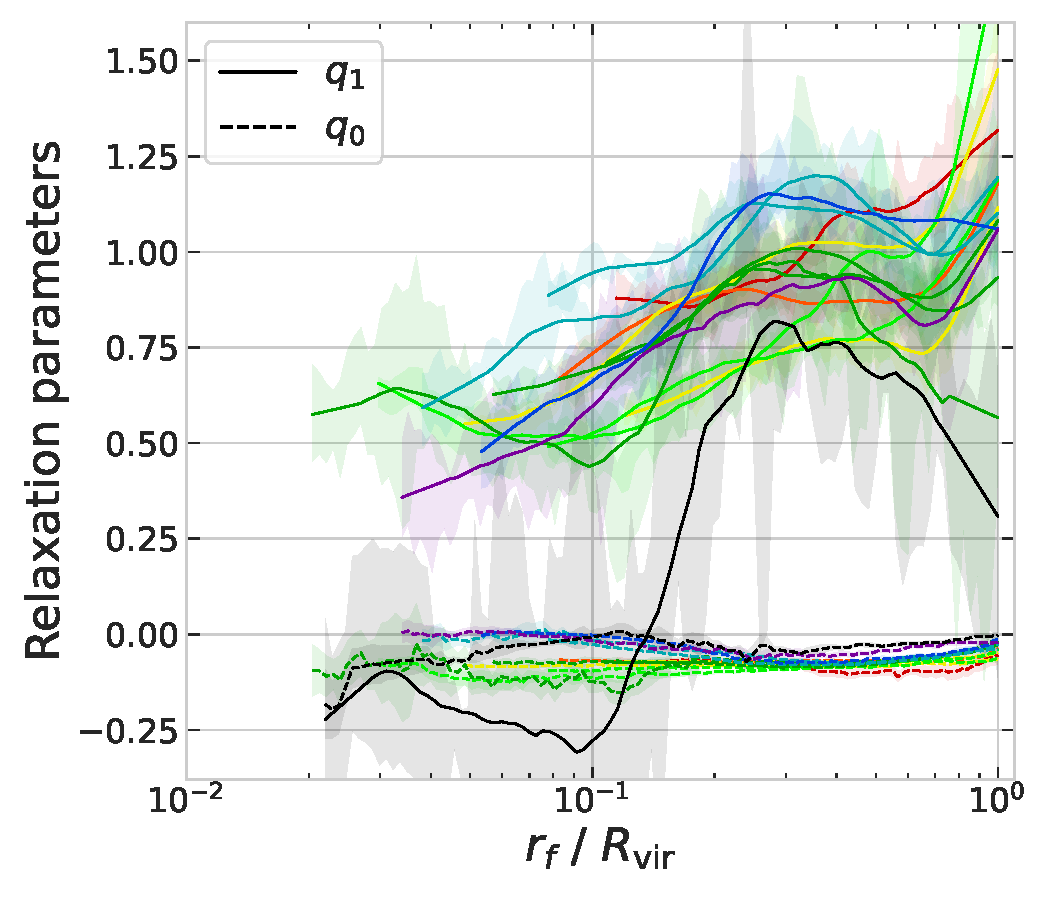
\includegraphics[width=0.48\linewidth,trim={0.5cm 0 0 0},clip]{plots/fit_params_rf_M_T_snap049.pdf}
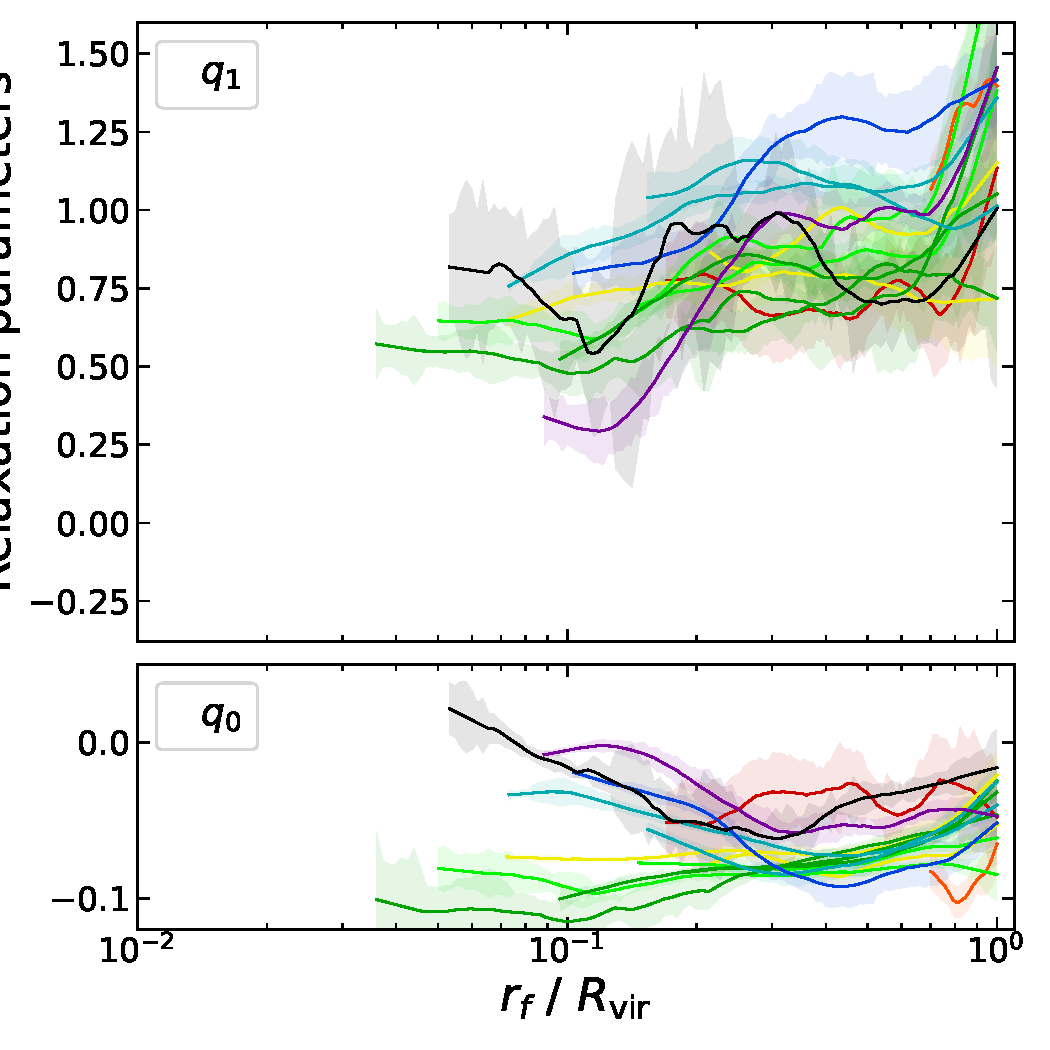
\includegraphics[width=0.48\linewidth,trim={0.5cm 0 0 0},clip]{plots/fit_params_rf_M_T_snap049_smpl98.pdf}
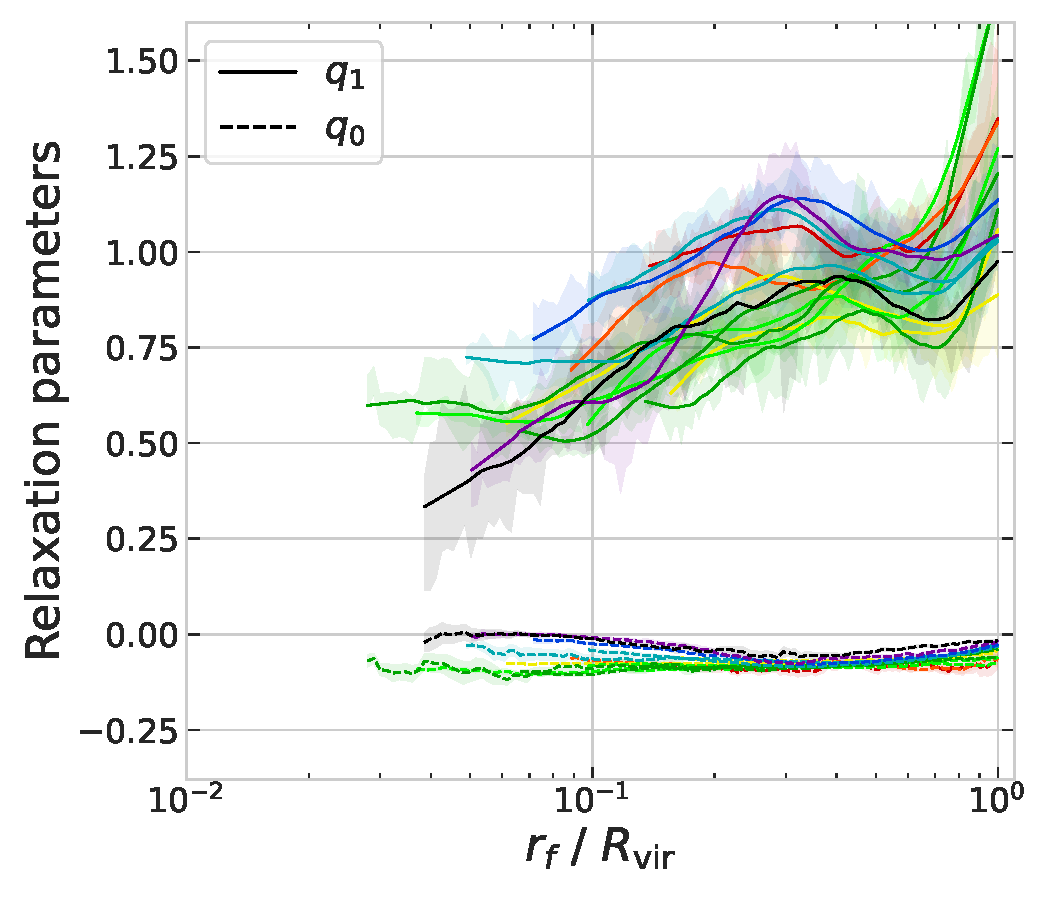
\includegraphics[width=0.48\linewidth,trim={0.5cm 0 0 0},clip]{plots/fit_params_rf_M_T_snap049_smpl98_allHalsMrange.pdf}
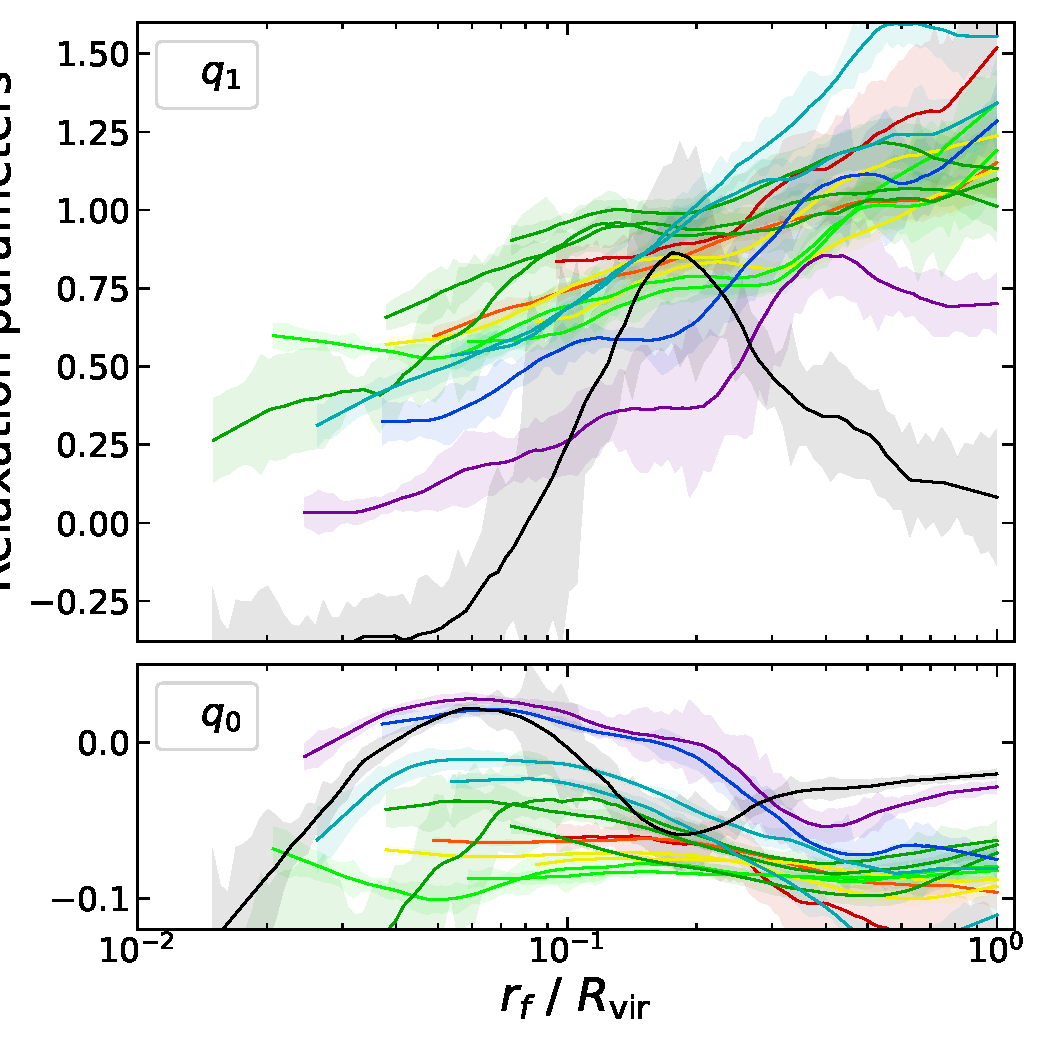
\includegraphics[width=0.48\linewidth,trim={0.5cm 0 0 0},clip]{plots/fit_params_rf_M_T_snap098.pdf}
\caption{Linear quasi-adiabatic relaxation model parameters $q_1$ and $q_0$ as a function of the halo-centric distance at different halo masses in IllustrisTNG at $z=0$ \emph{(bottom right panel)} and $z=1$ \emph{(other panels)}. In the top right panel, relaxation is shown at $z=1$ for the progenitors of the haloes selected at $z=0$. In the second row, left panel, relaxation is shown at different mass bins at $z=1$, indicated by corresponding mass bins at $z=0$. The color-coding follows Fig.~\ref{fig:mass_bin_label}.}
\label{fig:rf-fit-params}
\end{figure}

\begin{figure}[htbp]
\centering
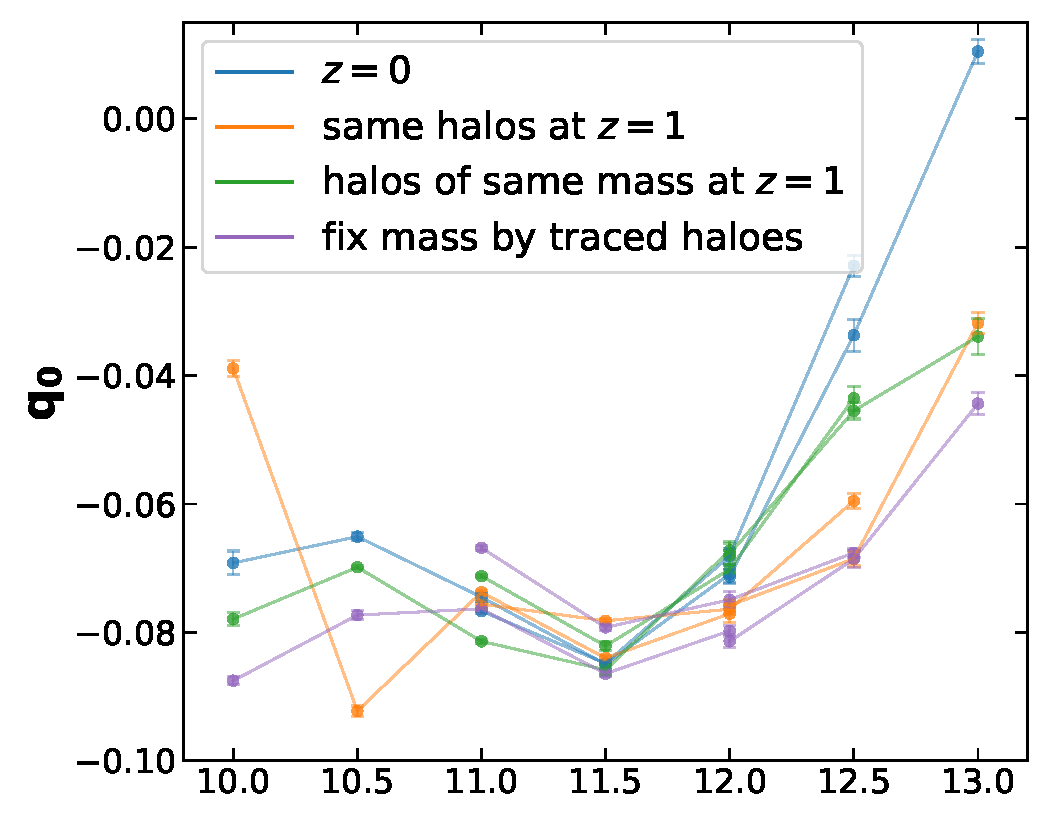
\includegraphics[width=0.6\linewidth]{plots/fit_param_q0_M_T_z01.pdf}
\caption{Mean of the radially dependent quasi-adiabatic relaxation offset, $q_{0}$ as a function halo mass in the four sets of halo samples indicated by color.}
\label{fig:fit-fit-func-q}
\end{figure}










\subsection{Variation in astrophysical feedback using CAMELS simulations}
\label{sec:res-physvar-CAMELS}
In this section, we present the role of various feedback parameters prescribed in the IllustrisTNG simulations using set of CAMELS simulations performed with the IllustrisTNG model. Let us first focus on the relaxation characterised by the intercepts in the relaxation relation of indvidual haloes. 

% \subsubsection*{Model independent relaxation offset}
For each matched halo, the y-intercept of the relaxation relation given by the relation between $M_i/M_f-1$ and $r_f/r_i-1$ is used to quantify the relaxation without modelling the relation. This parameter denoted as $q_y$ is the offset in the relaxation ratio $rf/ri$ from unity for the shells having a mass ratio of unity $M_i/M_f=1$. 

In particular, the x-intercept parameter $q_x$ is presented in the \figref{fig:camels-qx0} as a function of the astrophysical parameters in the CAMELS TNG set of simulations. We find that feedback strength parameters have a strong influence on the relaxation, however, the wind speed parameters have negligible effect on the relaxation characterized by $q_x$.

% The y-intercept of the relaxation relation is shown in \figref{fig:camels-qy0}.
Due to the limited resolution of the CAMELS simulation, the y-intercept of the relation was available only in smaller number of haloes. In other haloes, the mass ratios were always above one in the resolved outer regions of the halo. Hence we ignore the y-intercept.

 
 We then consider wider mass bins providing a few hundreds of haloes within the small volume of the CAMELS simulation. Using the radially dependent relation analysis we have obtained the $q_0(r_f)$ and study its mean across the halo. This is presented in \figref{fig:camels-qoq1}. We find that at $z=1$, the magnitude of $q_0$ is larger with stronger AGN feedback indicated by larger $A_{\rm{AGN1}}$. However this trend is absent is totally absent in $z=0$. This could be because of a strong suppression in star formation rate at present epoch due to the stronger AGN feedback in the past.
\begin{figure}[htbp]
\centering
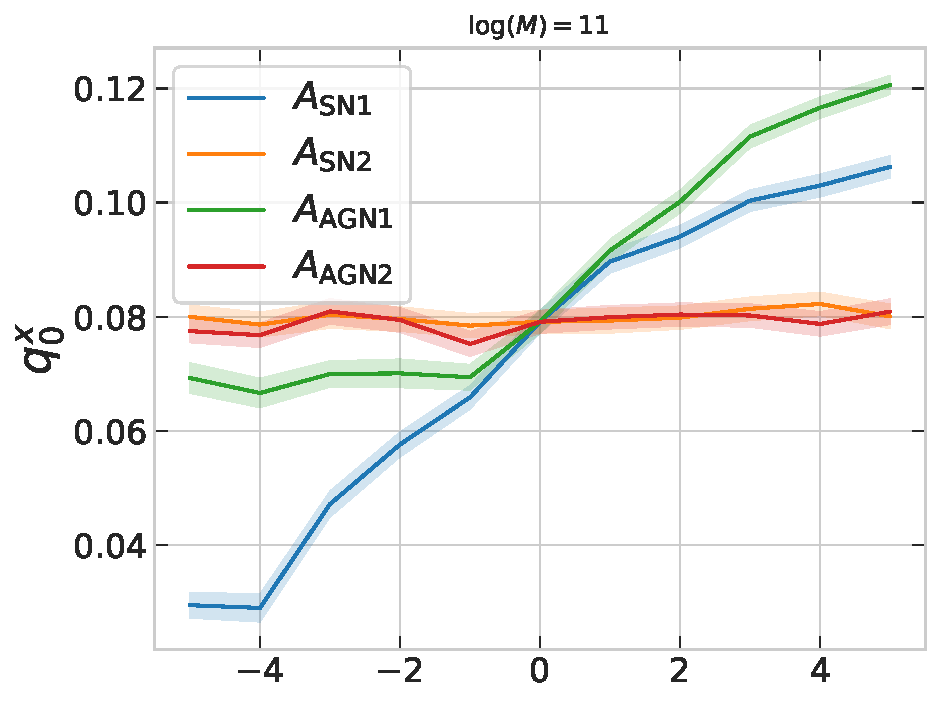
\includegraphics[width=0.325\linewidth]{plots/CAMELS_I_qx0_sn18_11.pdf}
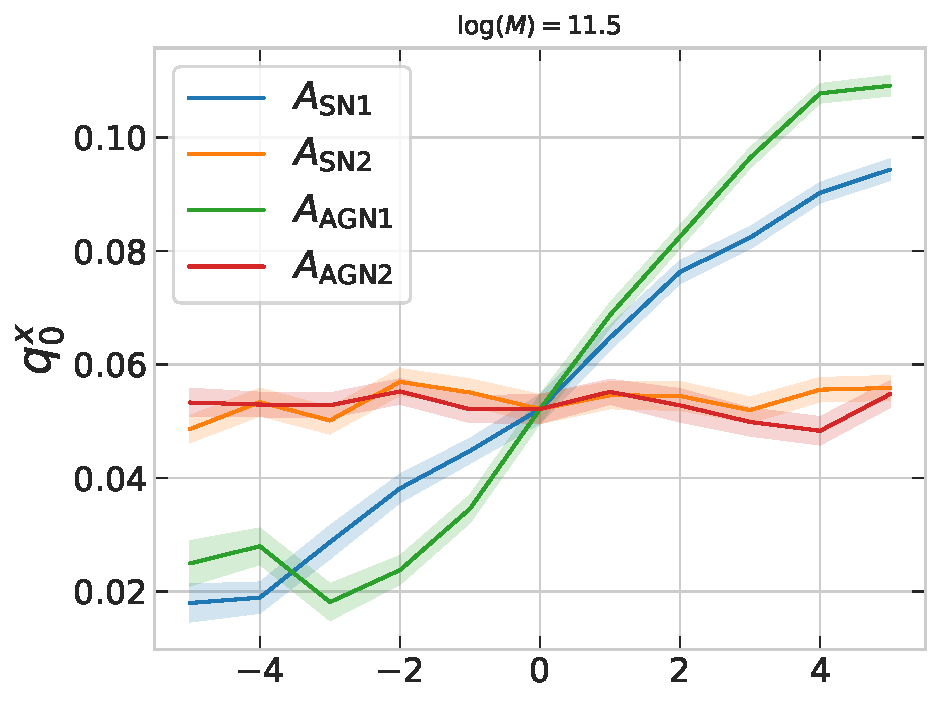
\includegraphics[width=0.325\linewidth]{plots/CAMELS_I_qx0_sn18_11.5.pdf}
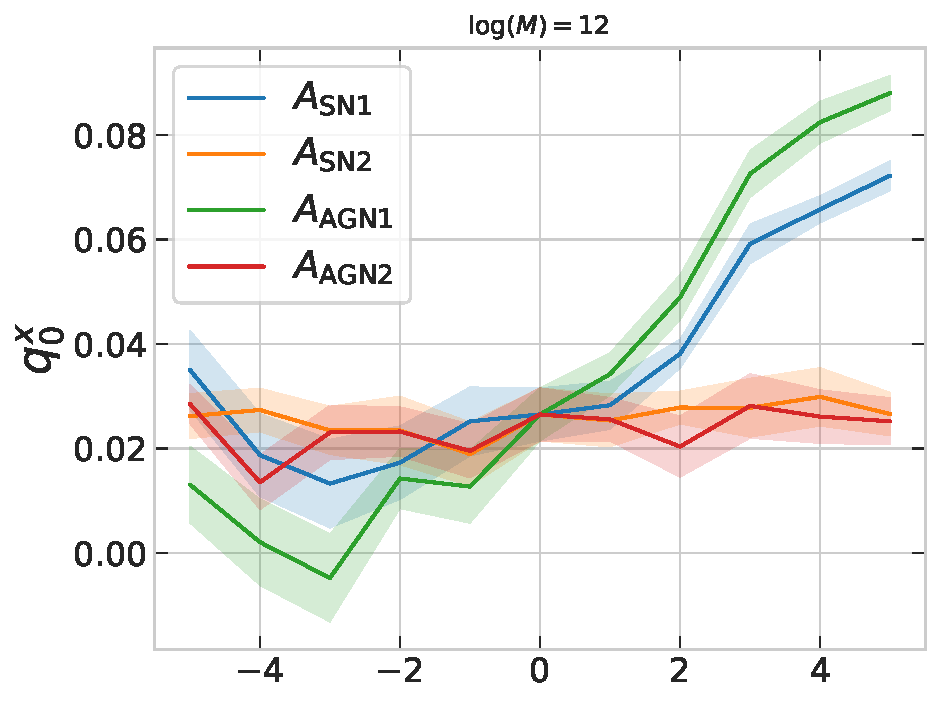
\includegraphics[width=0.325\linewidth]{plots/CAMELS_I_qx0_sn18_12.pdf}
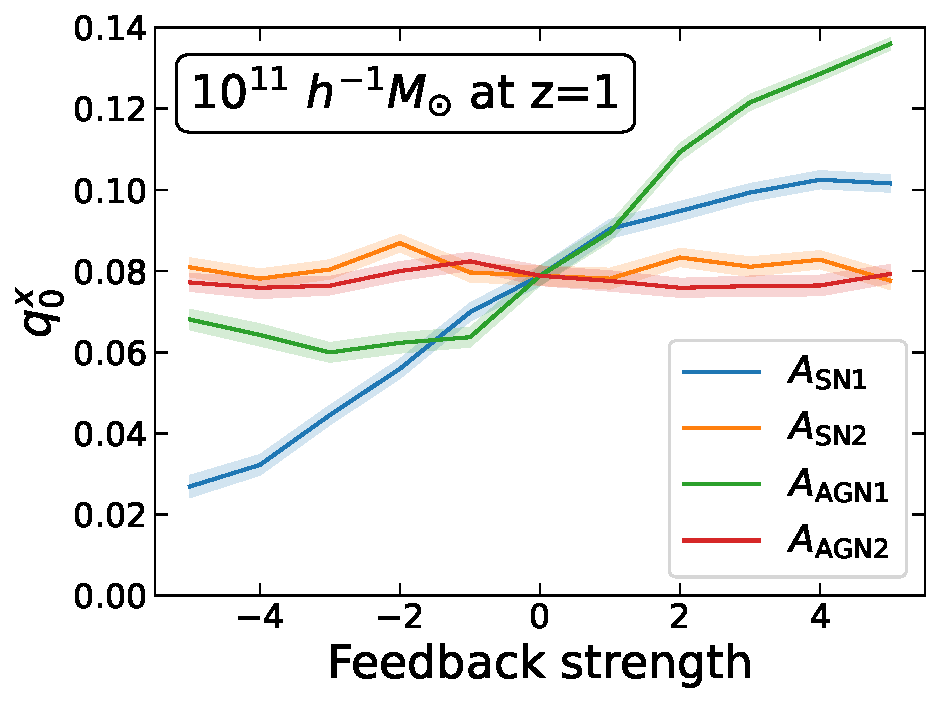
\includegraphics[width=0.325\linewidth]{plots/CAMELS_I_qx0_sn33_11.pdf}
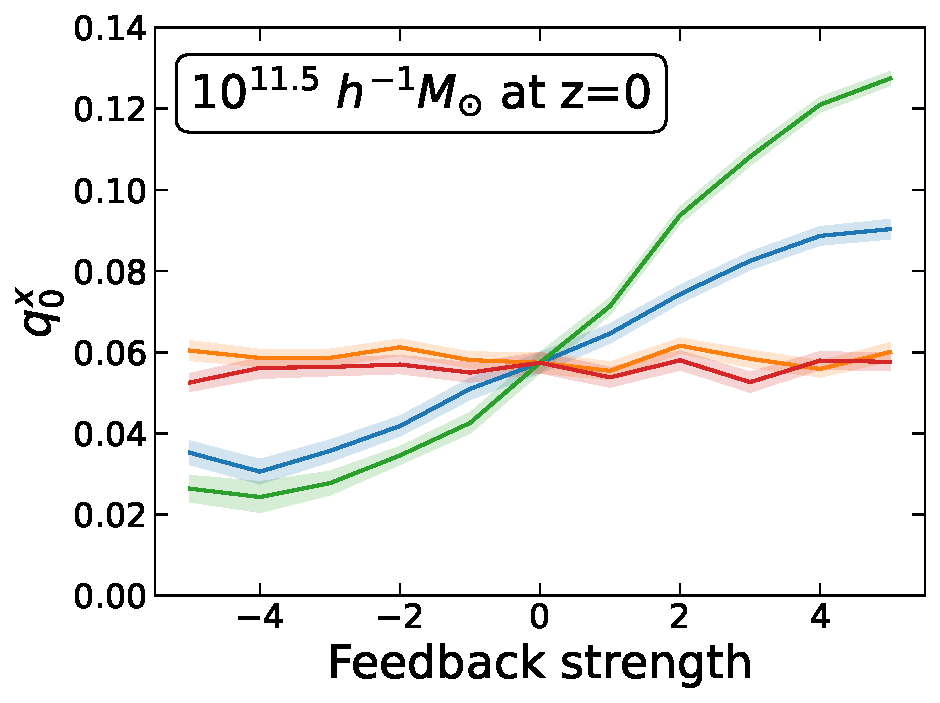
\includegraphics[width=0.325\linewidth]{plots/CAMELS_I_qx0_sn33_11.5.pdf}
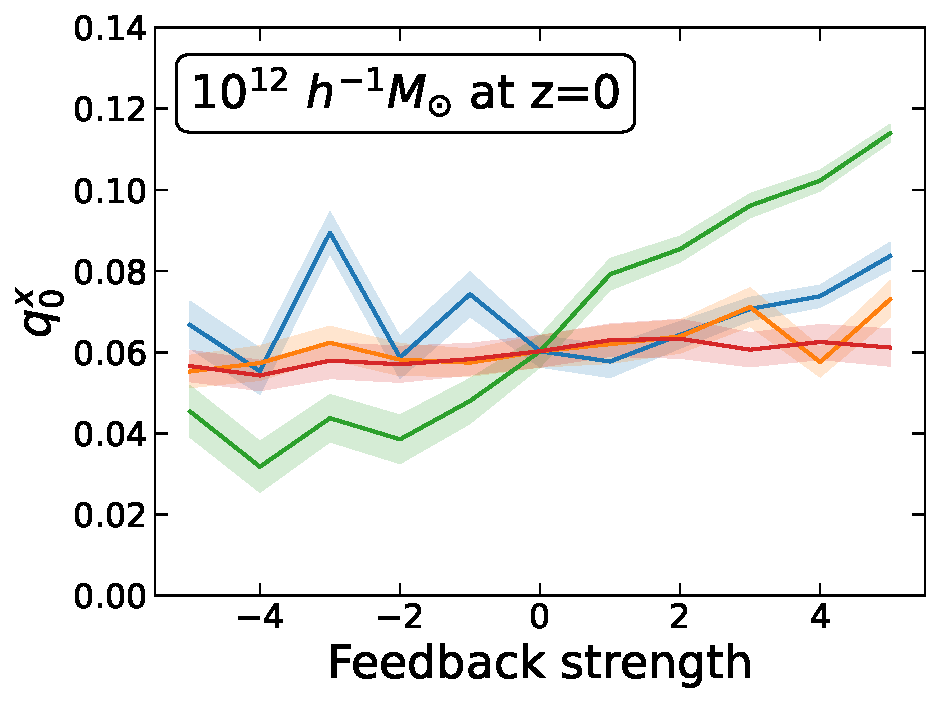
\includegraphics[width=0.325\linewidth]{plots/CAMELS_I_qx0_sn33_12.pdf}
\caption[]{Response as a function of the baryonic feedback parameters in CAMELS-TNG. Top: z=1, Bottom: z=0}
\label{fig:camels-qx0}
\end{figure}


% \begin{figure}[htbp]
% \centering
% 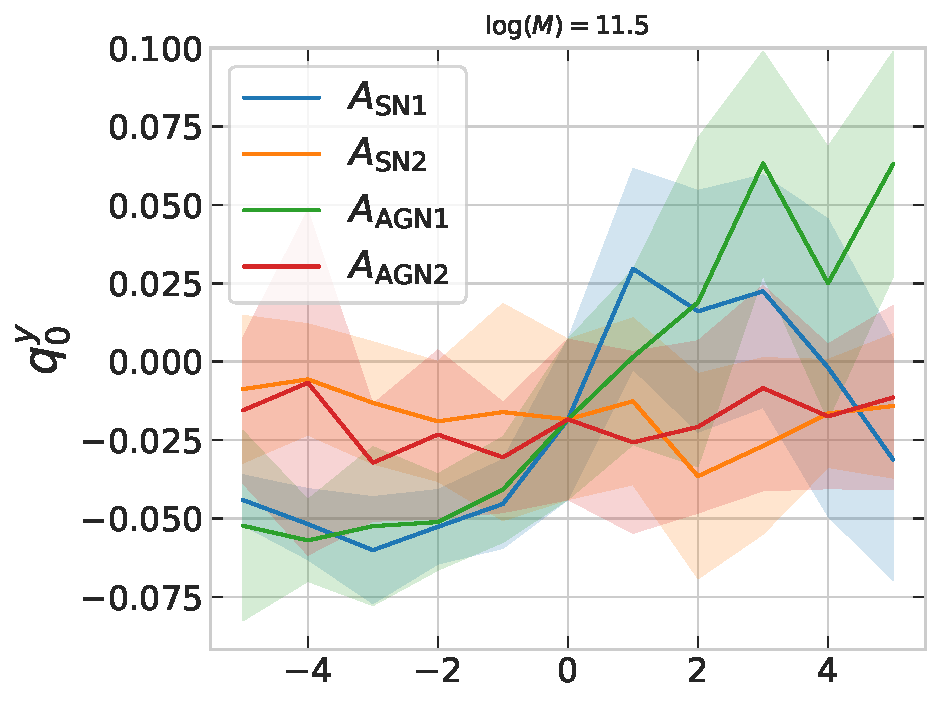
\includegraphics[width=0.325\linewidth]{plots/CAMELS_I_qy0_sn18_11.5.pdf}
% 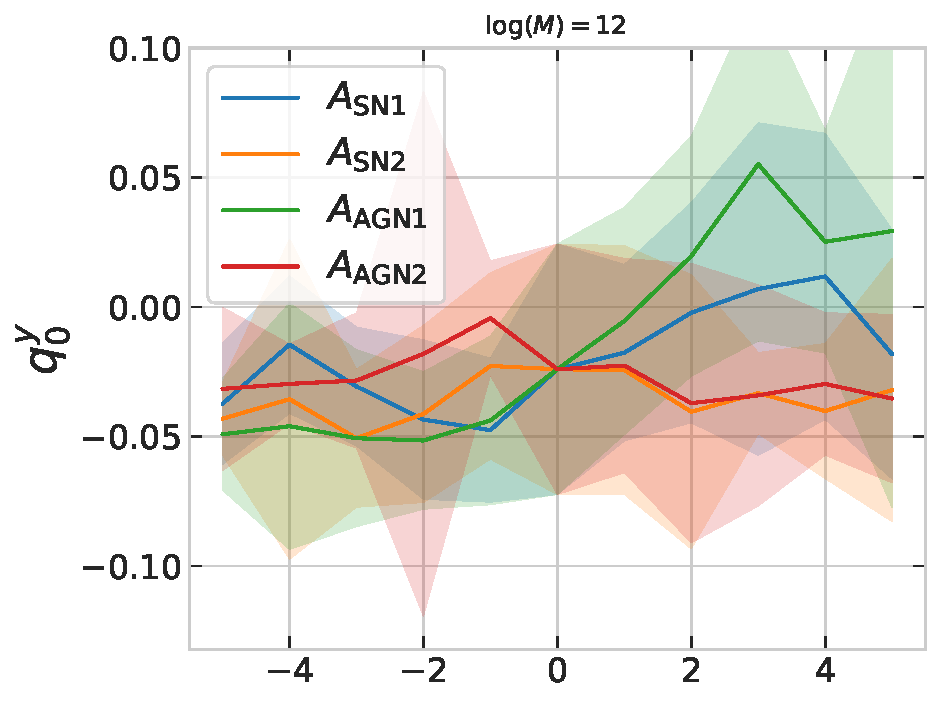
\includegraphics[width=0.325\linewidth]{plots/CAMELS_I_qy0_sn18_12.pdf}
% 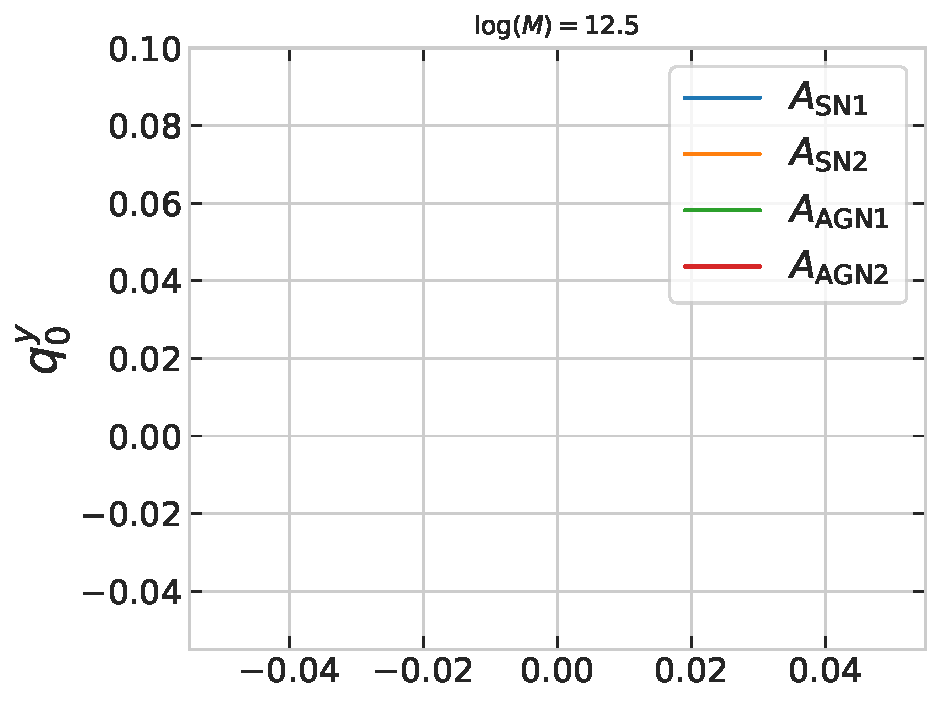
\includegraphics[width=0.325\linewidth]{plots/CAMELS_I_qy0_sn18_12.5.pdf}
% 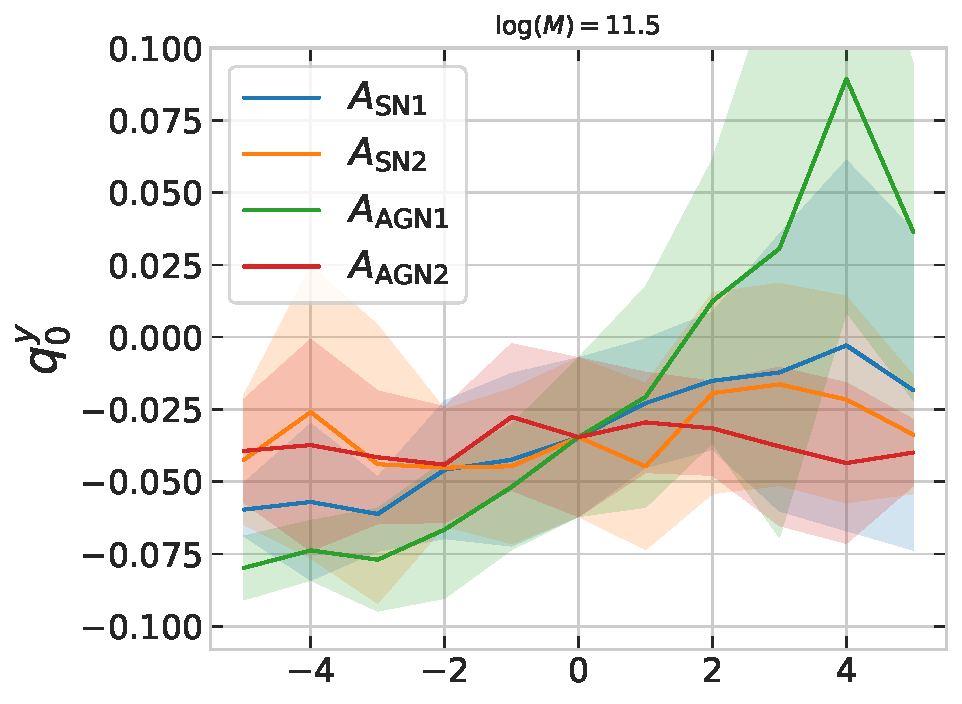
\includegraphics[width=0.325\linewidth]{plots/CAMELS_I_qy0_sn33_11.5.pdf}
% 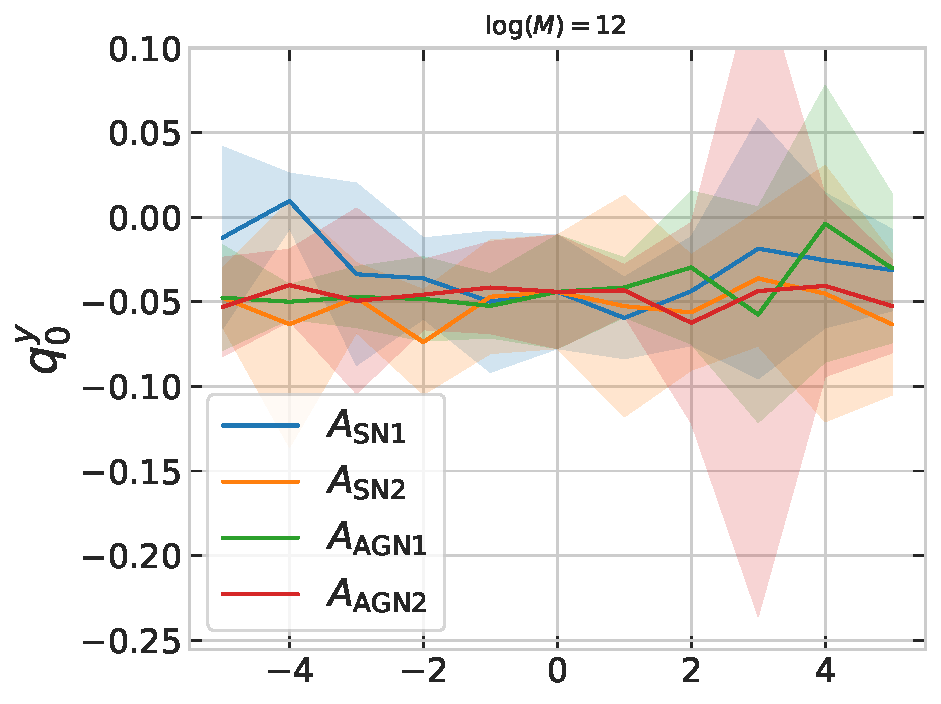
\includegraphics[width=0.325\linewidth]{plots/CAMELS_I_qy0_sn33_12.pdf}
% 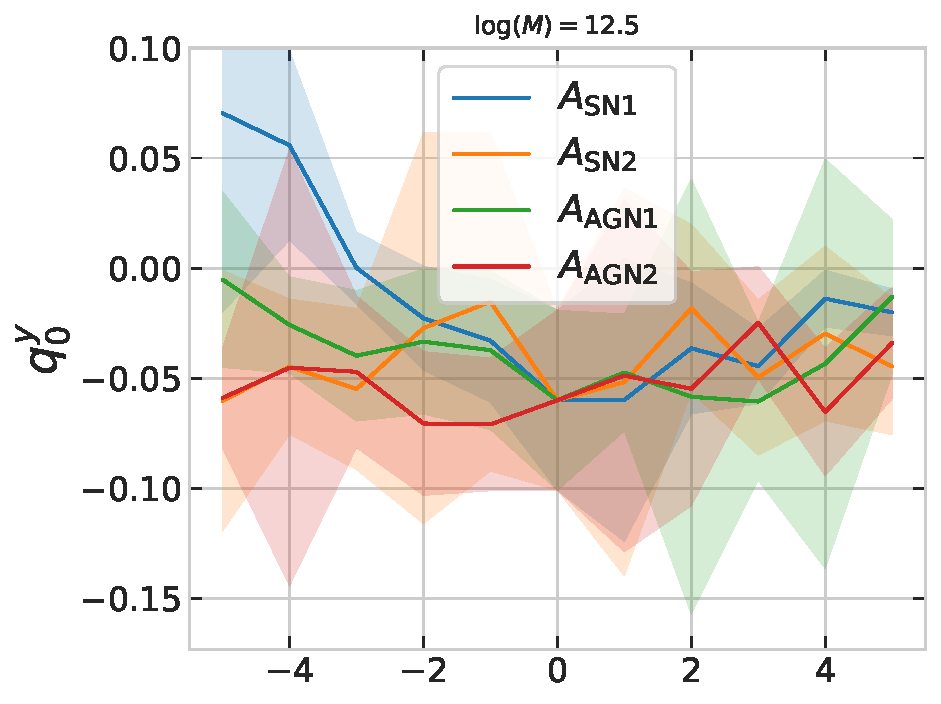
\includegraphics[width=0.325\linewidth]{plots/CAMELS_I_qy0_sn33_12.5.pdf}
% \caption[]{Response as a function of baryonic parameters in CAMELS-TNG. \\\hspace{\textwidth}Top: $z=1$, Bottom: $z=0$.}
% \label{fig:camels-qy0}
% \end{figure}
\begin{figure}[htbp]
\centering
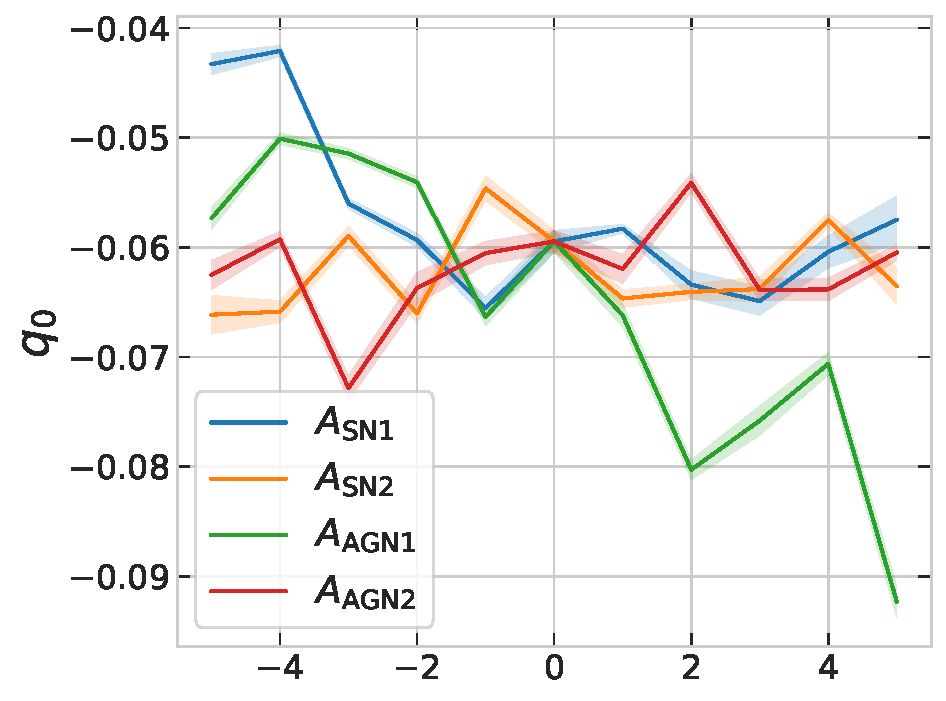
\includegraphics[width=0.49\linewidth]{plots/CAMELS_I_q0_sn18.pdf}
% 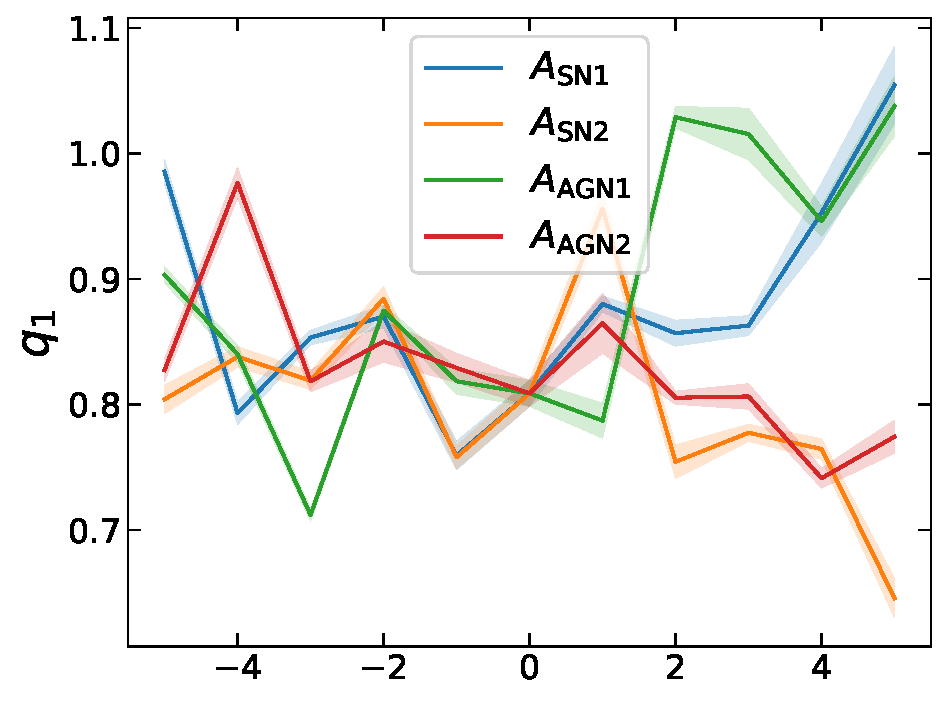
\includegraphics[width=0.49\linewidth]{plots/CAMELS_I_q1_sn18.pdf}
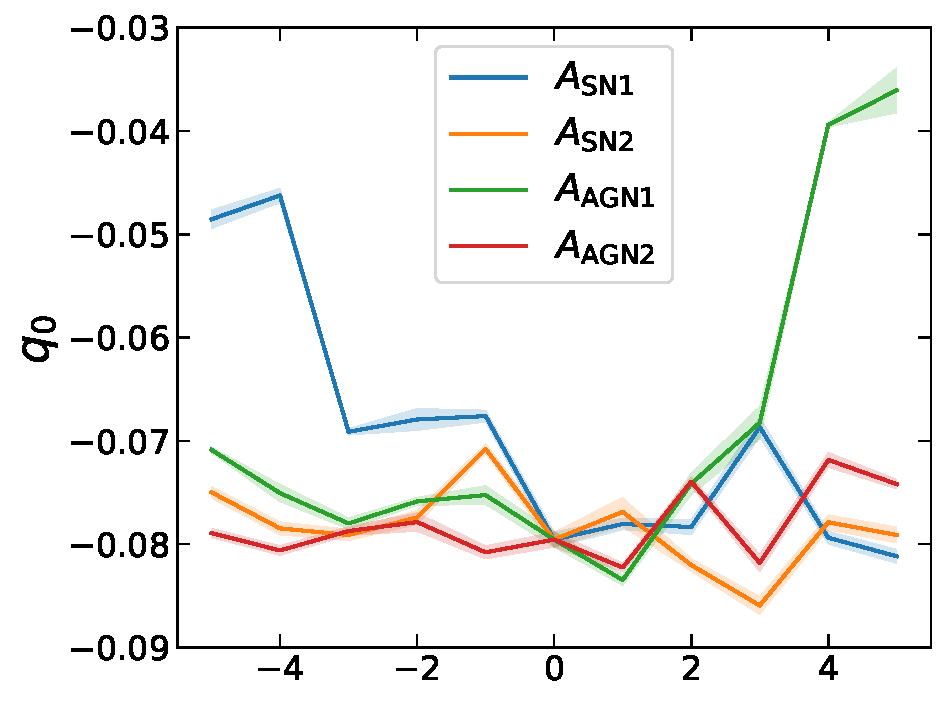
\includegraphics[width=0.49\linewidth]{plots/CAMELS_I_q0_sn33.pdf}
% 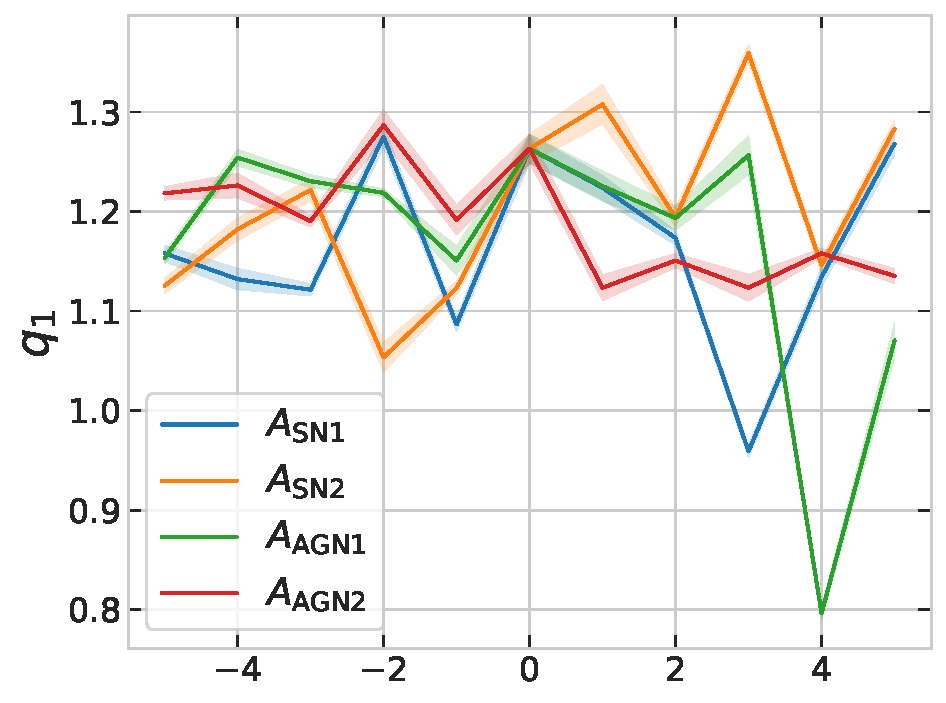
\includegraphics[width=0.49\linewidth]{plots/CAMELS_I_q1_sn33.pdf}
\caption[]{Response as a function of the baryonic feedback parameters in CAMELS-TNG. Left: $z=1$, Right: $z=0$.}
\label{fig:camels-q0q1}
\end{figure}









\subsection{Role of astrophysical models in EAGLE simulations}
\label{sec:res-physvar-eagle}
In this section, we present insights from small boxes of EAGLE simulations on the role of different feedback mechanisms on the relaxation response.
Due to the significantly smaller box size, we don't get enough haloes to obtain a radially dependent relaxation relation for large haloes, so for such haloes, we only present the radially independent stacked relaxation relation; This is shown in \figref{fig:EAGLE-rad-indep}. We find that among all the variations, the gas equation of state has a stronger impact on the relaxation relation. In particular, the `eos53' simulation shows strong expansion of the dark matter halo in response to galaxy formation.

% \begin{figure}[htbp]
% \centering
% 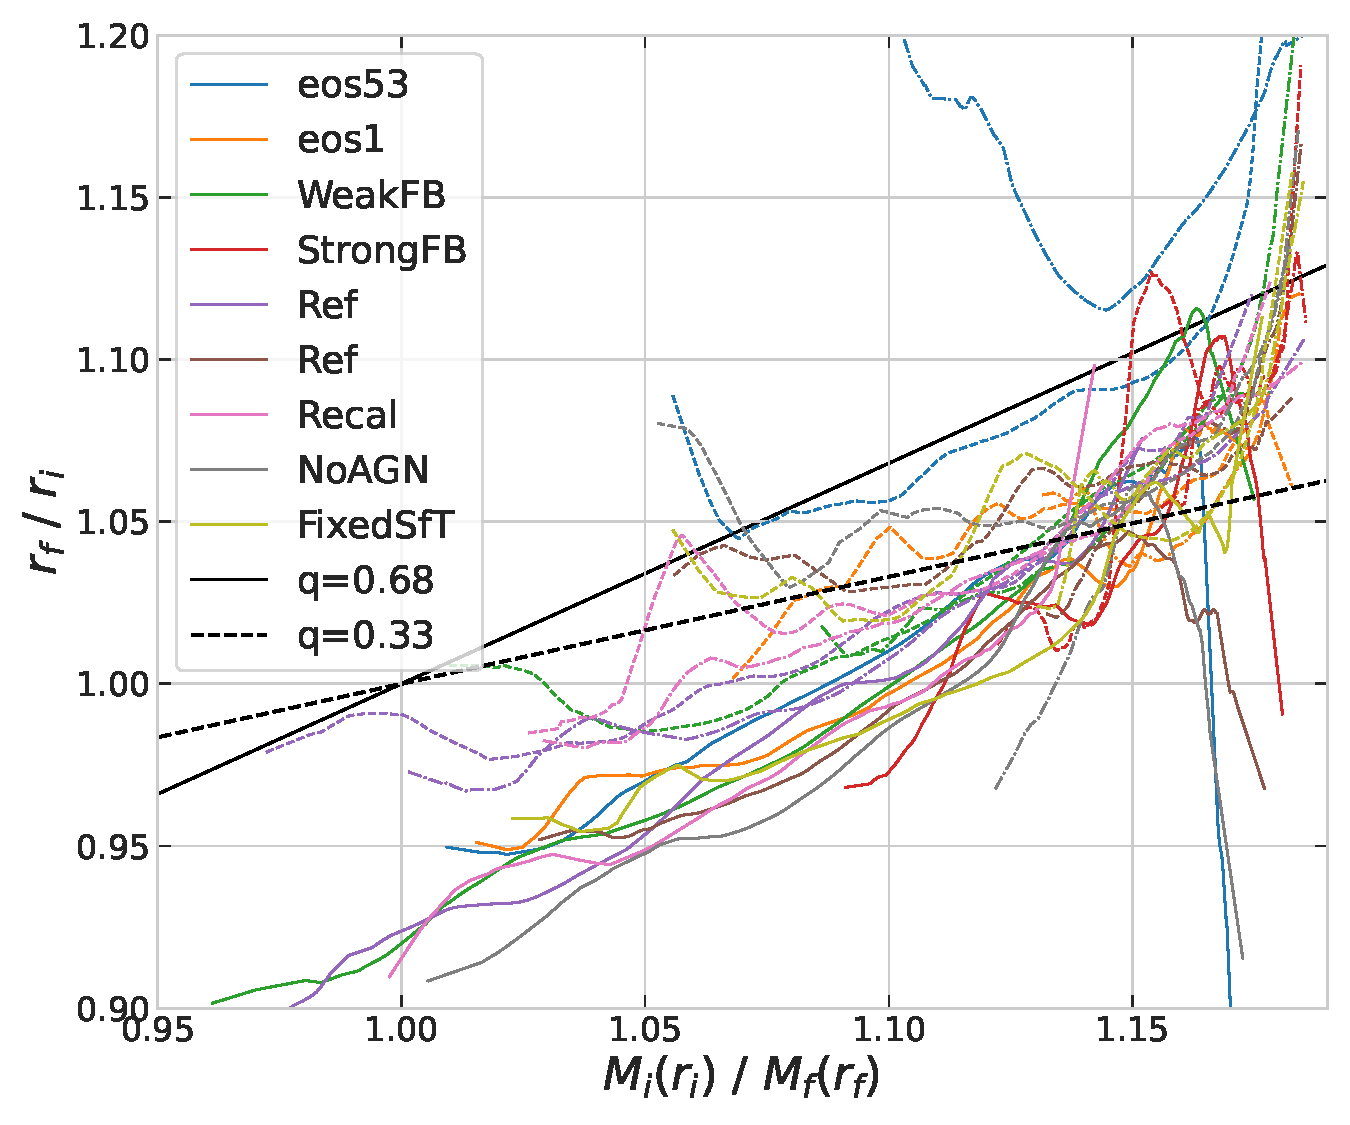
\includegraphics[width=.75\linewidth]{plots/eagle_physvar_rad_indep_relxn_reln_MiMf_all.pdf}
% 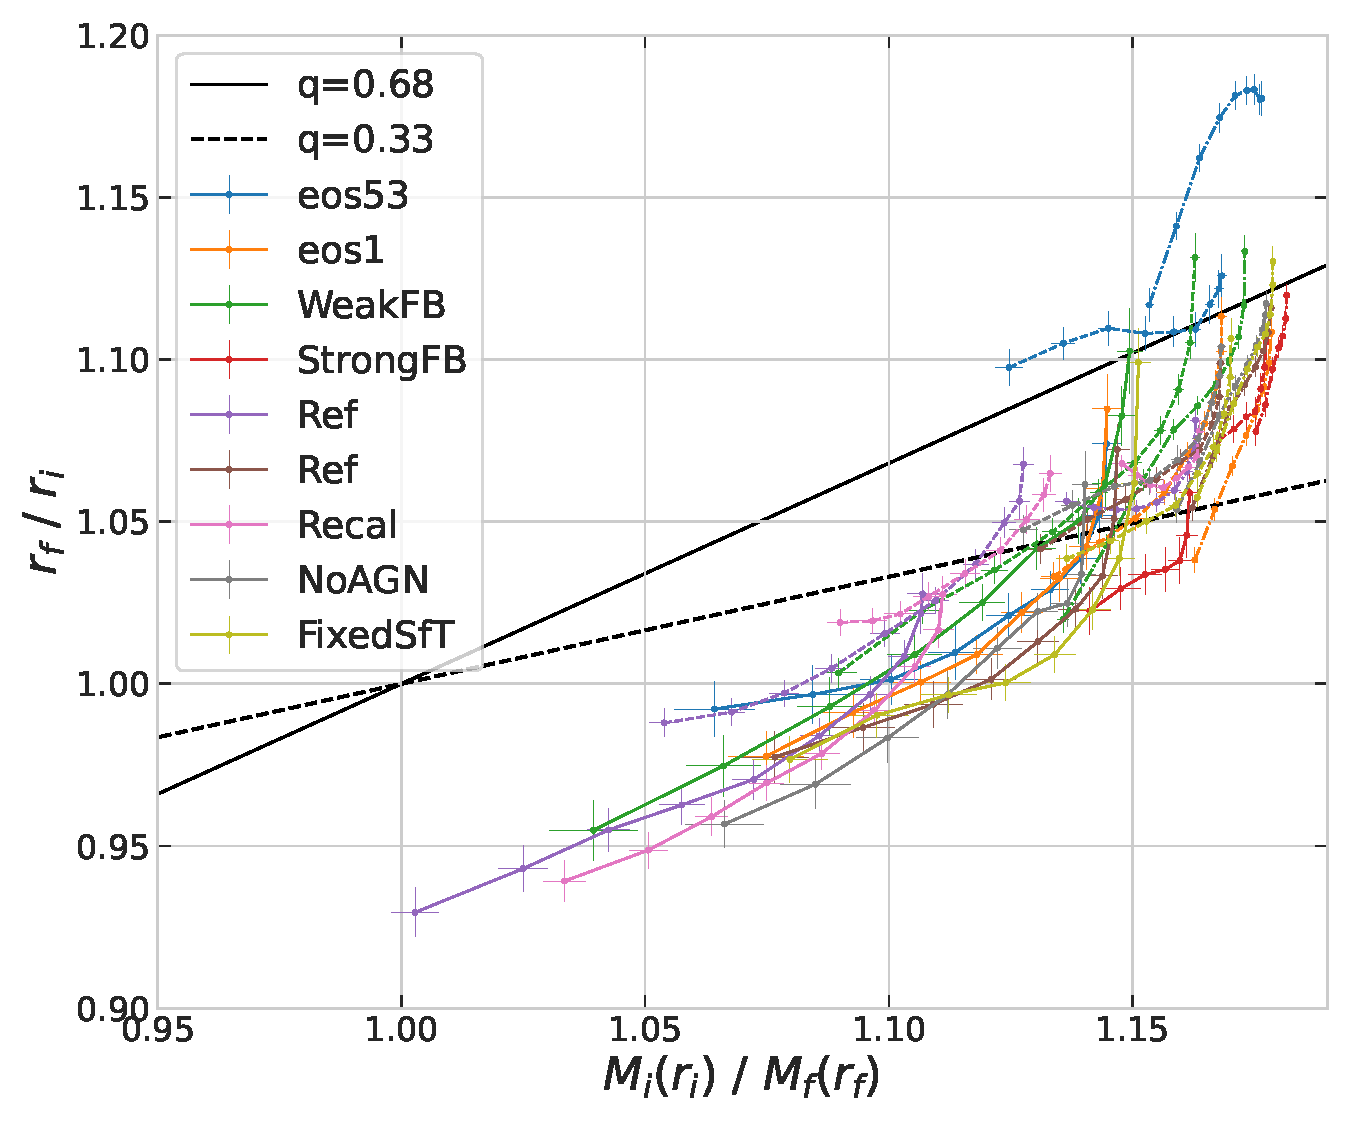
\includegraphics[width=.75\linewidth]{plots/eagle_physvar_rad_indep_relxn_reln_rf_all.pdf}
% \caption[]{Relaxation as a function of baryonic physics prescription in EAGLE simulation.  \PV{See next figure for clarity}}
% \end{figure}

\begin{figure}[htbp]
\centering
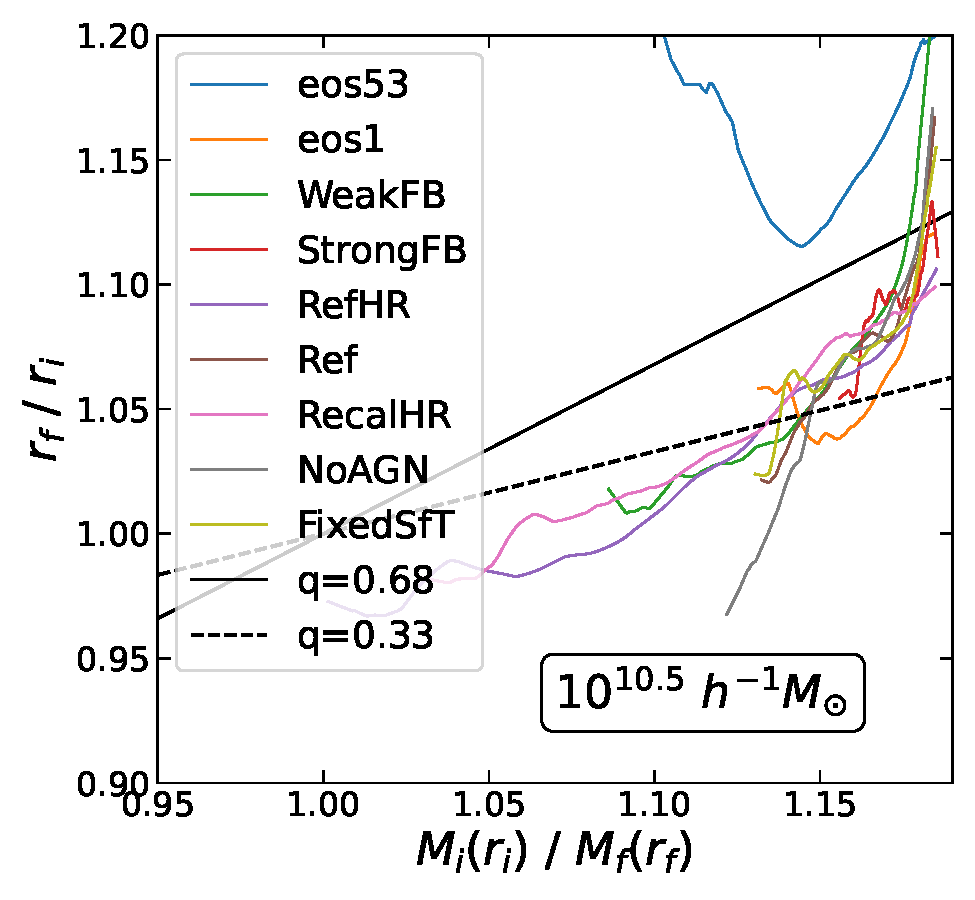
\includegraphics[width=0.32\linewidth]{plots/eagle_physvar_rad_indep_relxn_reln_MiMf_10.5.pdf}
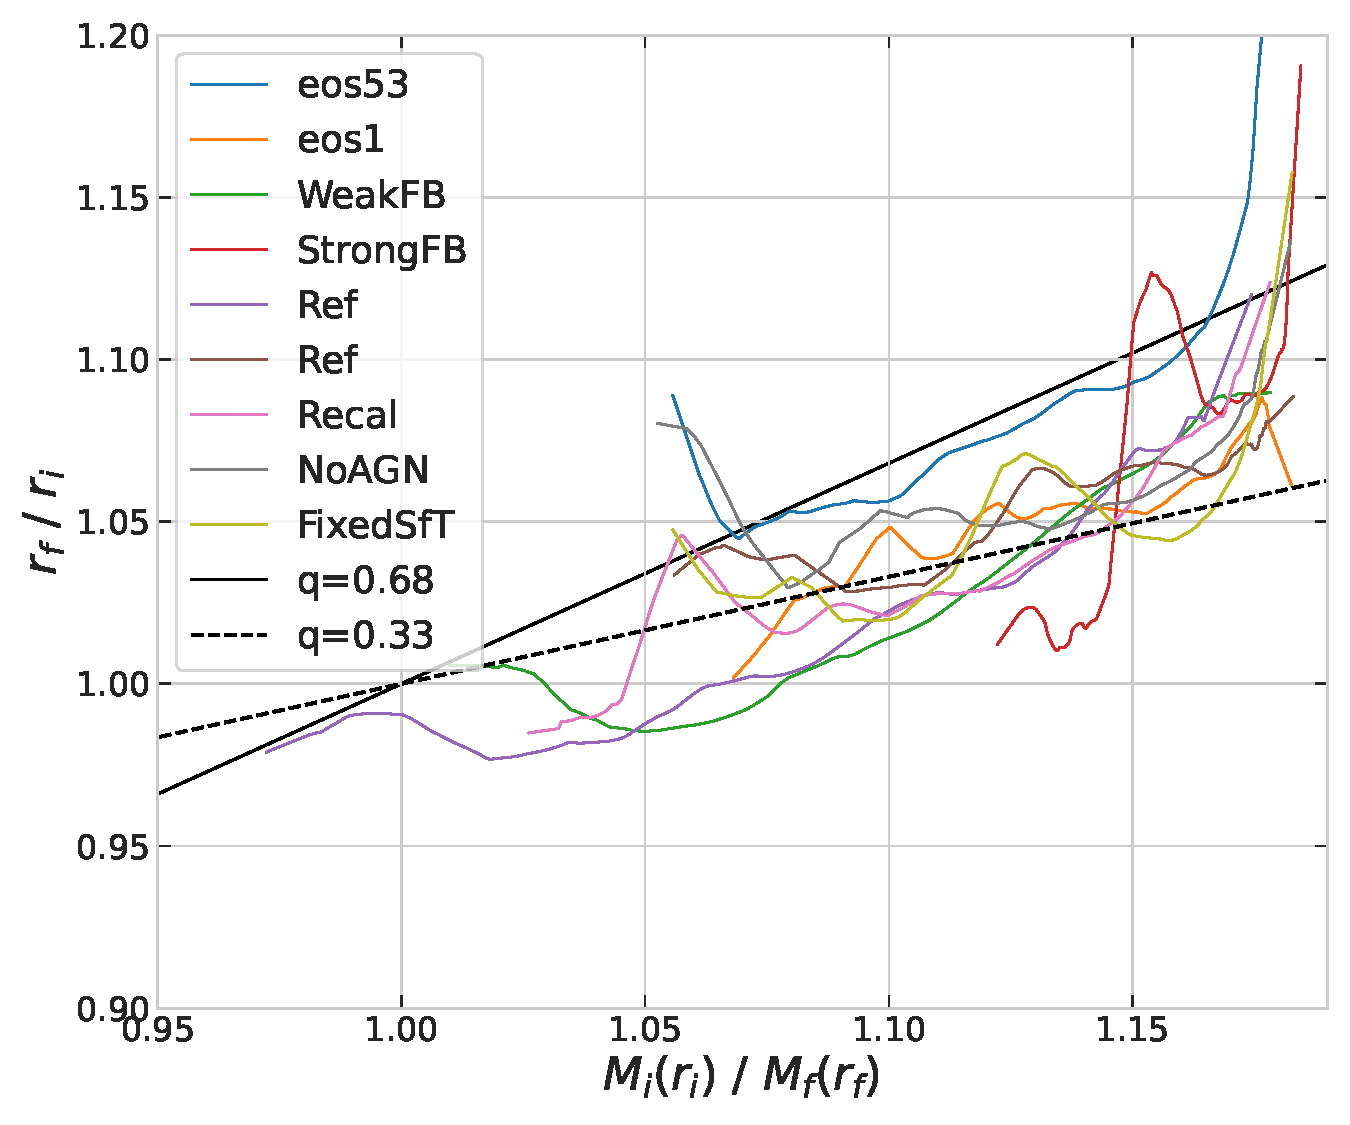
\includegraphics[width=0.32\linewidth]{plots/eagle_physvar_rad_indep_relxn_reln_MiMf_11.pdf}
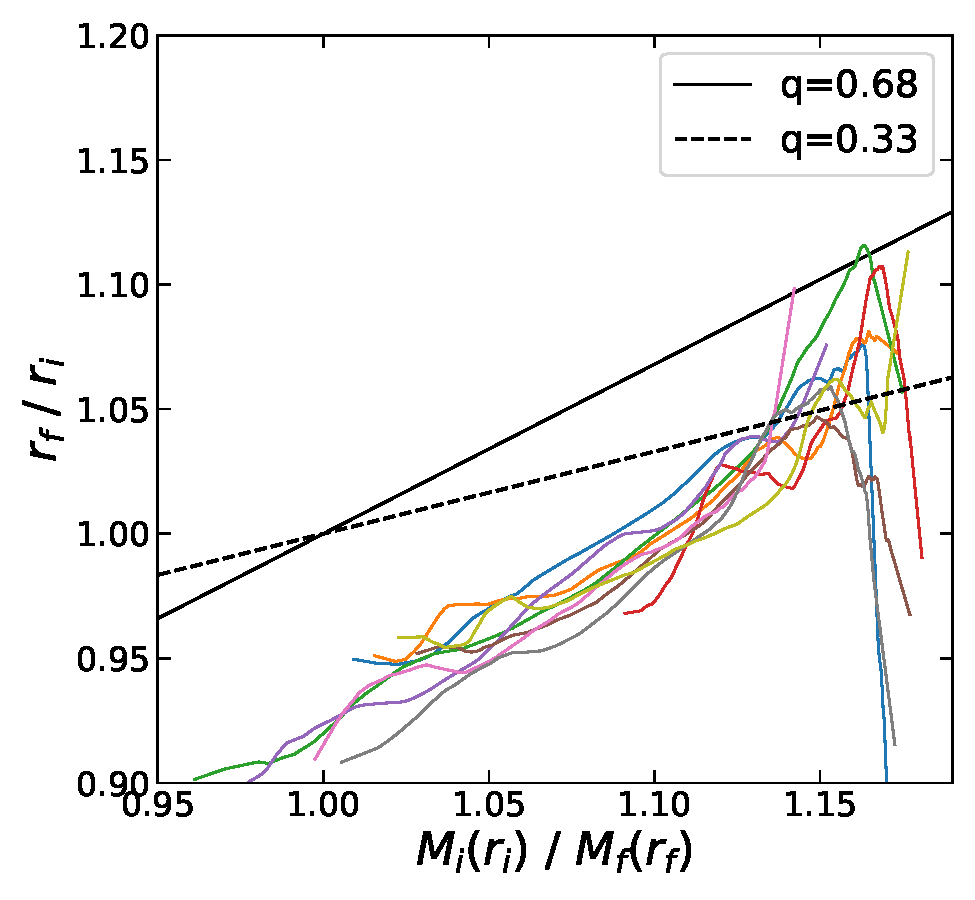
\includegraphics[width=0.32\linewidth]{plots/eagle_physvar_rad_indep_relxn_reln_MiMf_11.5.pdf}
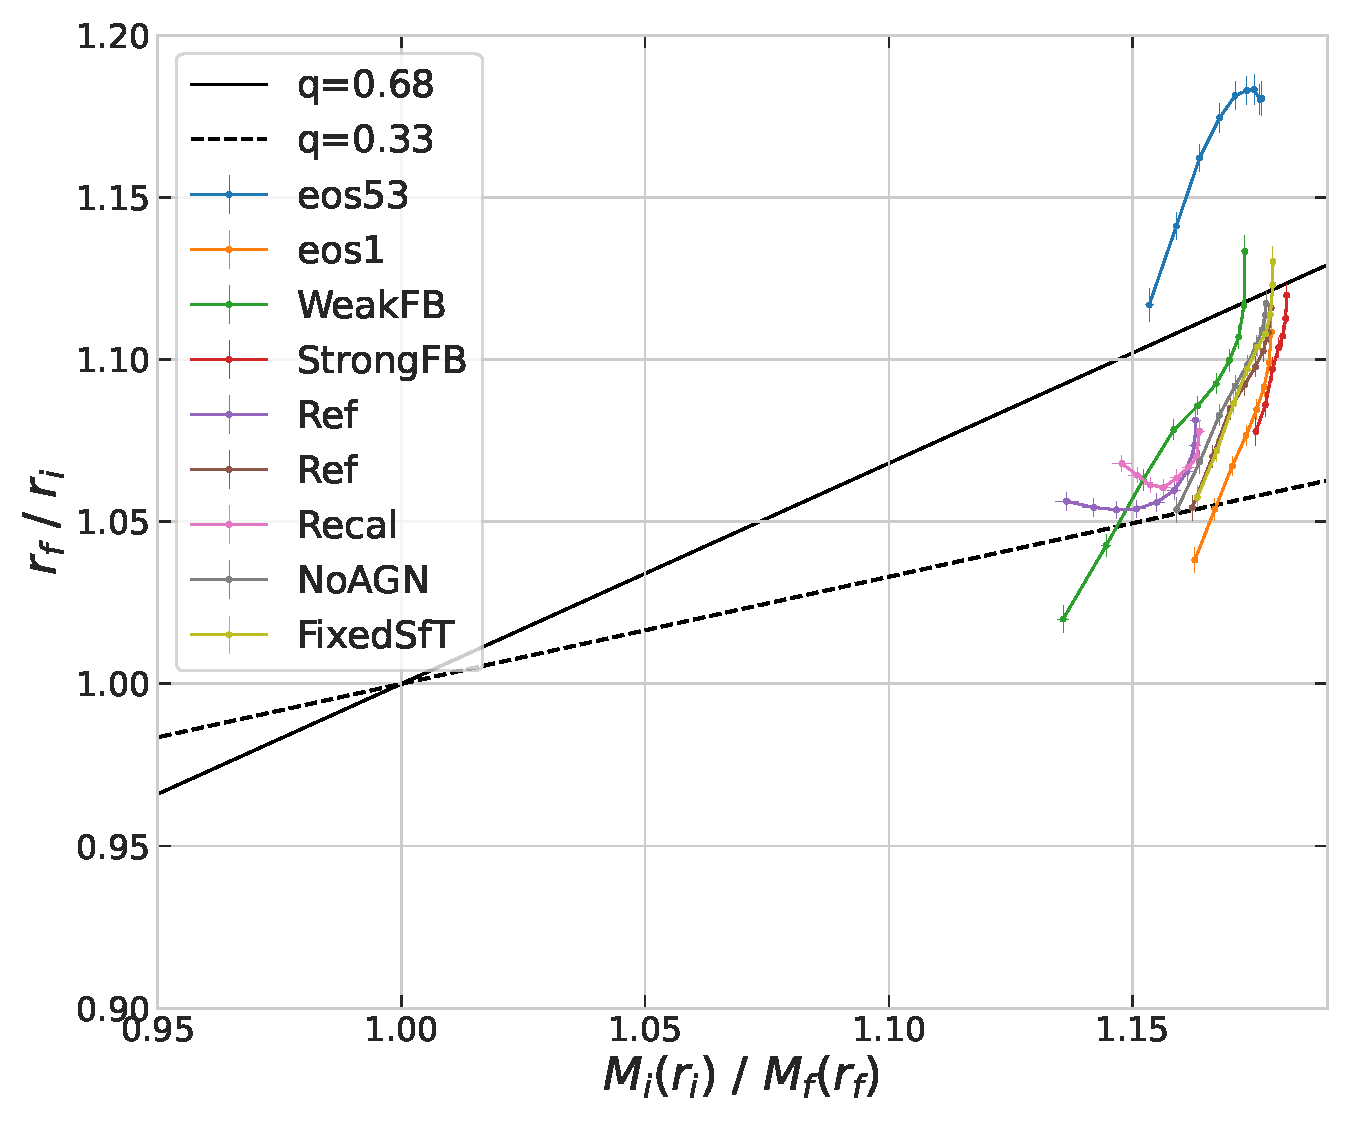
\includegraphics[width=0.32\linewidth]{plots/eagle_physvar_rad_indep_relxn_reln_rf_10.5.pdf}
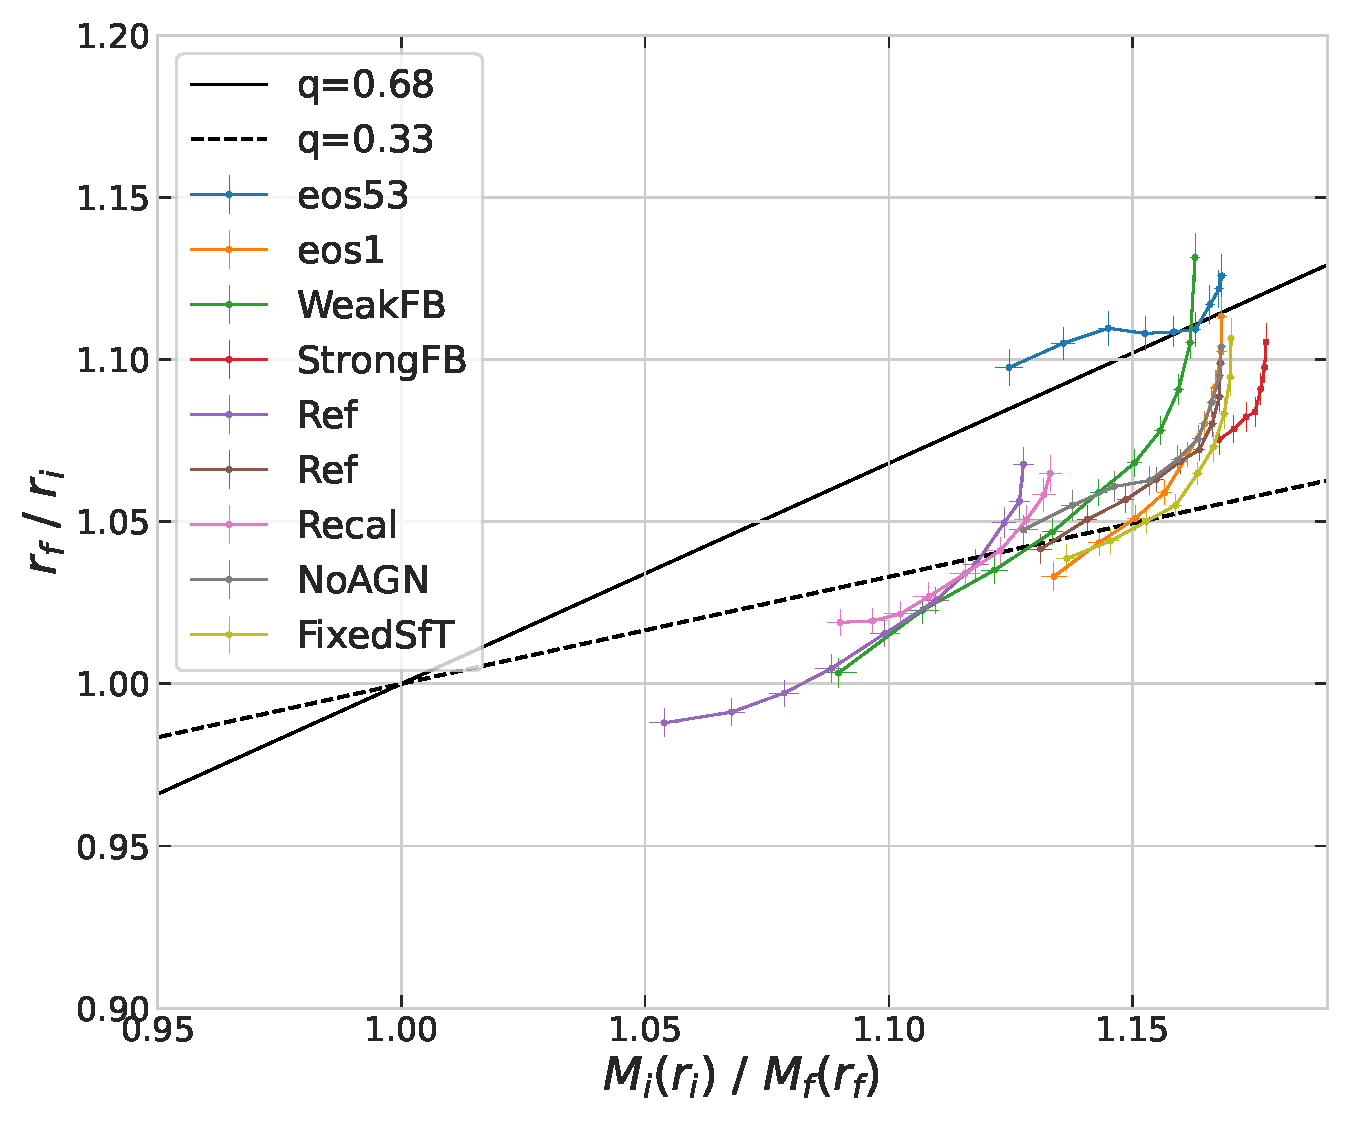
\includegraphics[width=0.32\linewidth]{plots/eagle_physvar_rad_indep_relxn_reln_rf_11.pdf}
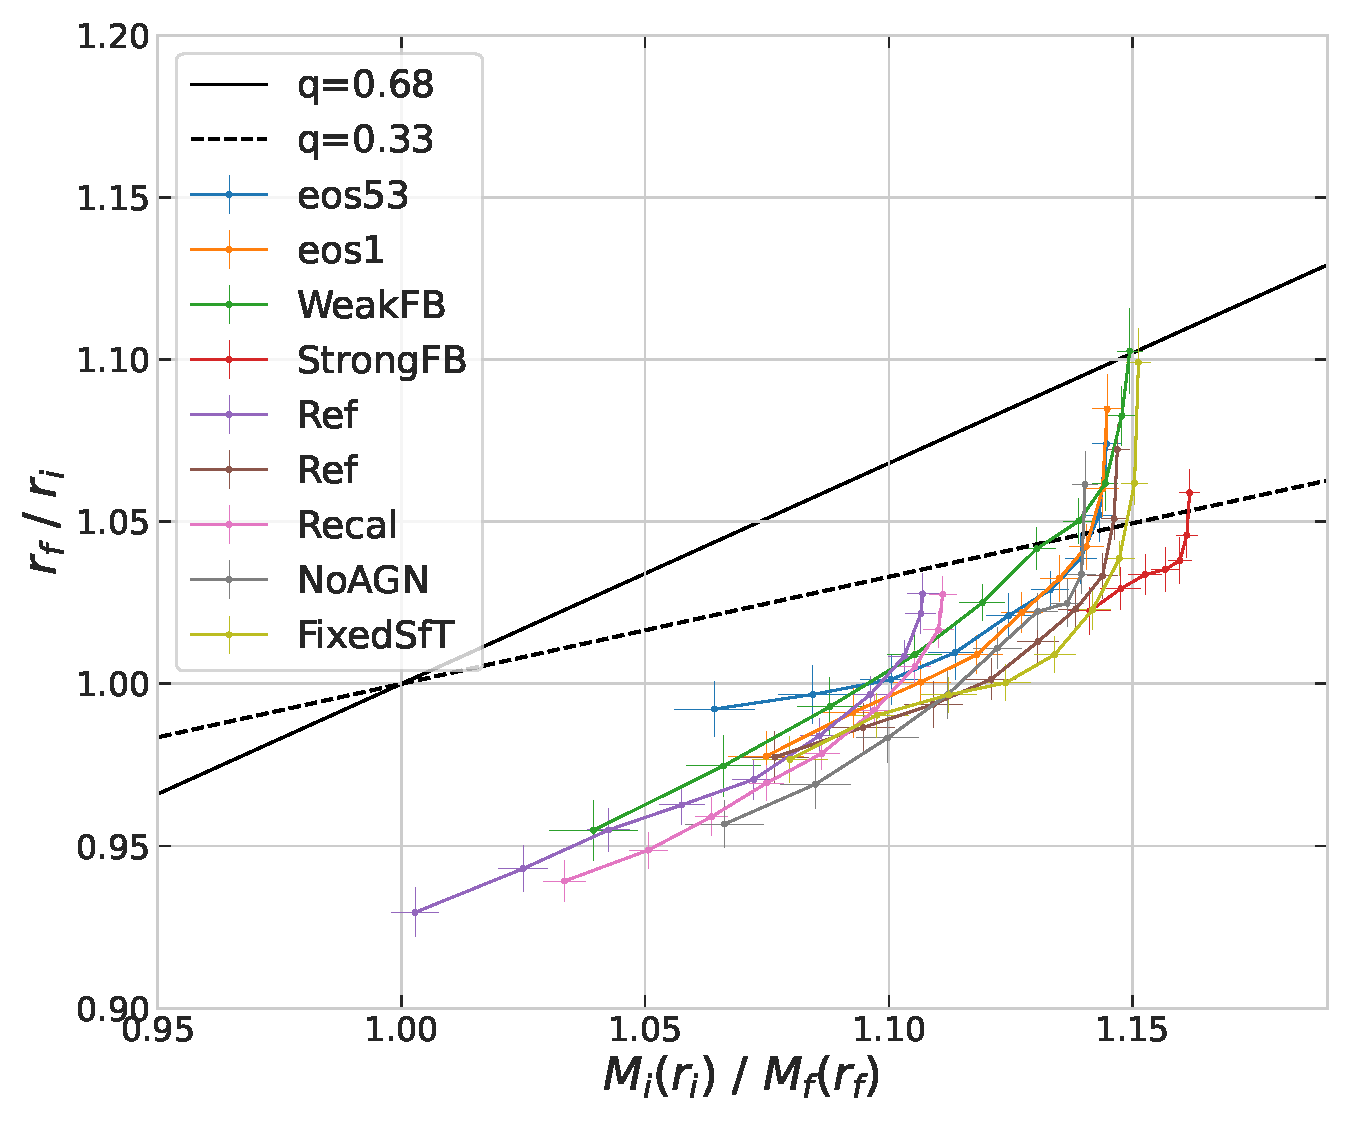
\includegraphics[width=0.32\linewidth]{plots/eagle_physvar_rad_indep_relxn_reln_rf_11.5.pdf}
\caption[]{Relaxation as a function of baryonic physics prescription in EAGLE simulation for haloes at low-mass haloes from $10^{10.5} \Mh$ to $10^{11.5} \Mh$. In the top panels, the relaxation relation is stacked at fixed mass ratios independent of the radius; while they are stacked at fixed halo-centric radii in the lower panels.}
\label{fig:EAGLE-rad-indep}
\end{figure}

\begin{figure}[htbp]
\centering
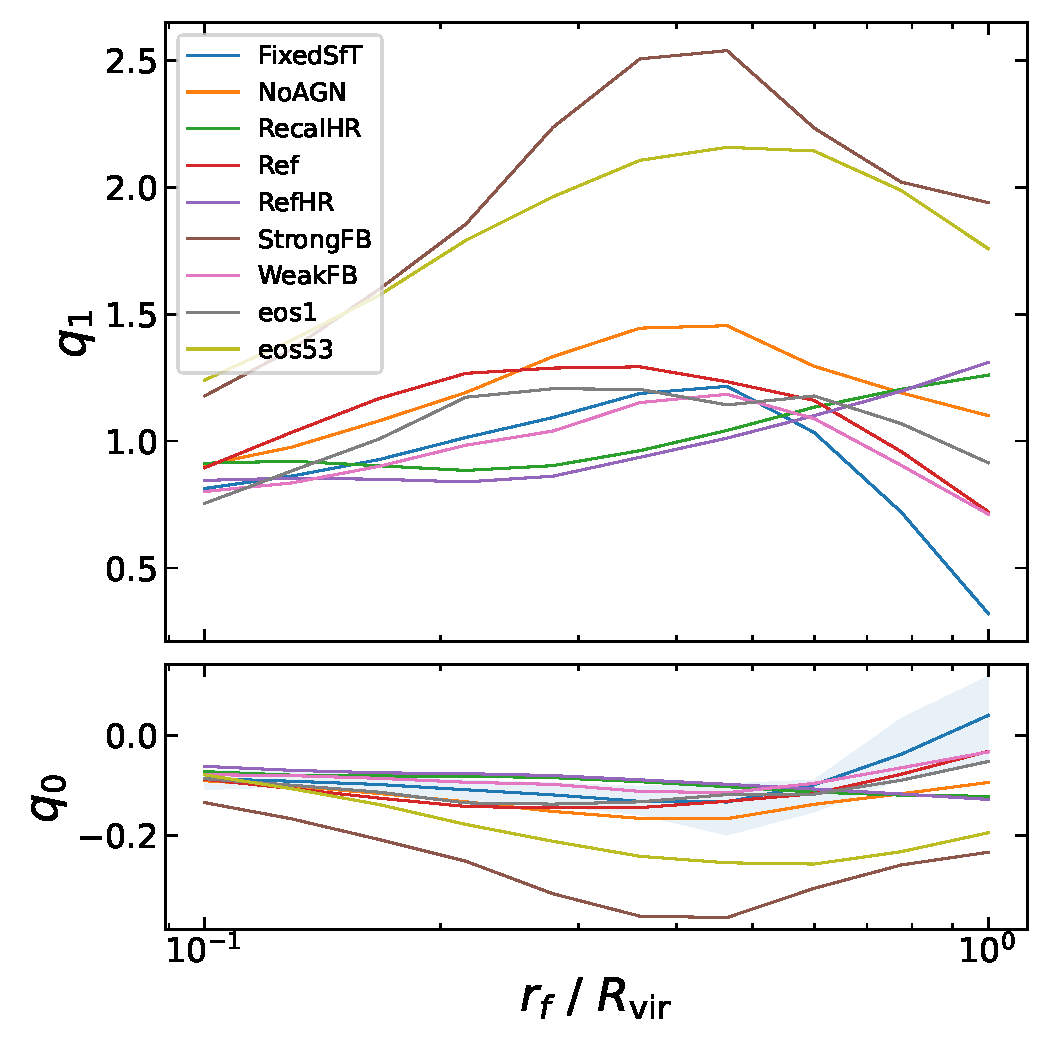
\includegraphics[width=0.7\linewidth]{plots/fit_params_rf_M_E_physvar_fatmass_uniradb.pdf}
\caption[]{Relaxation as a function of baryonic physics prescription in the EAGLE simulation.}
\end{figure}


\section{Conclusion}
\label{sec:conclusion}
% In this work, we have studied the relaxation response of dark matter halo in simulation with variation in the baryonic astrophysics and at different epoch. 
% \begin{itemize}
%     \item Through IllustrisTNG simulations, we found that the relaxation is significantly different at $z=1$ from the $z=0$. This difference could not be accounted by a simple halo property such as its mass or the peak height.
%     \item Through EAGLE simulations we found that the equation of state of gas plays a significant role in determining the halo relaxation response.
% \end{itemize}


In this chapter, We investigated the influence of astrophysical modeling on the relaxation response of dark matter haloes at different epochs, specifically focusing on \( z=0 \) and \( z=1 \). The analysis is divided into three main parts, each shedding light on the role of various astrophysical processes in shaping the dark matter content of haloes.

% \subsubsection*{1. Early Epoch in IllustrisTNG Simulations}
We began by examining the relaxation response at an earlier redshift (\( z=1 \)) in the IllustrisTNG simulations using three distinct set of halo samples, which highlight the variations in relaxation across different halo masses. Our study reveals that dark matter relaxation tends to be usually stronger (smaller \(r_f/r_i\)) at the earlier epoch compared to the present among haloes of the same mass. This is even more prominent among the progenitors of present epoch haloes. Notably, we observe that cluster-scale haloes at \( z=1 \) show significant relaxation (\(r_f/r_i<1\)) that is also a function of the change in the enclosed mass (\(M_i/M_f\)). This is in contrast to similar haloes at the present epoch, where \(r_f/r_i\) stayed close to unity on average irrespective of the value of \(M_i/M_f\).

We also find that the locally linear quasi-adiabatic relaxation model is also a good description of the relaxation relation at this earlier epoch, demonstrating its robustness in capturing the dark matter response across redshifts. Moreover, the parameters of the radially dependent relaxation are found to be more universal across a much wider range of masses at \( z=1 \). For example, the progenitors of even the most massive clusters are well characterized by the simple three-parameter model of relaxation that was developed with a focus on galactic-scale haloes at \( z=0 \).

% \subsubsection*{2. Variation in Astrophysical Feedback Using CAMELS Simulations}
Next, we explore variations in astrophysical feedback strengths within the IllustrisTNG model using simulations from the CAMELS project, which varies four different feedback parameters: two for stellar feedback and two for AGN feedback. Our analysis shows that the parameters controlling the energy flux of the feedback have a significant impact on the relaxation of dark matter at different epochs. In contrast, the parameters governing the speed and burstiness of feedback have negligible effects on the halo relaxation response.

We find that variations in stellar feedback strengths have a larger impact among dwarf galaxy-scale haloes, while variations in AGN feedback parameters exert a stronger influence on Milky Way-scale haloes. Notably, the relaxation offset in the outer well-resolved regions is stronger at the present epoch than at \( z=1 \), contrasting with results from the inner regions explored in the IllustrisTNG simulations in the first part of this chapter.

The stronger implementation of AGN feedback tends to result in greater relaxation at both \( z=0 \) and \( z=1 \) in the outer regions of the haloes. However, in the slightly inner regions, stronger AGN feedback implementation leads to a weaker relaxation offset at \( z=0 \) and a stronger offset at \( z=1 \). We interpret this as a consequence of the overall reduction in total feedback at \( z=0 \) due to the suppression of star formation caused by higher AGN feedbacks in the past. These results highlight the significance of feedback mechanisms in building a physical understanding of dark matter halo relaxation.

% \subsubsection*{3. Role of Astrophysical Models in the EAGLE Simulations}
Finally, we assess the impact of different astrophysical models in the EAGLE simulations. Supernova feedback strengths show a similar trend to that observed in the CAMELS simulations. Additionally, we find that the gas equation of state has the strongest effect on the relaxation response of dark matter, particularly among haloes hosting dwarf galaxies.

Overall, this chapter underscores the intricate relationship between baryonic processes and dark matter halo relaxation, illustrating the variations that arise due to different astrophysical models and redshifts.